\documentclass[a4paper,12pt]{article}

\usepackage{amssymb}
\usepackage{amsmath}
\usepackage{amsthm}
\usepackage{graphicx}
\usepackage{color}

\usepackage{cancel}
\usepackage{hyphenat}

\definecolor{palpurp}{rgb}{.49,.19,.48}

\author{B. C. Dobbs}
\title{Minimal Surfaces in $\mathbb R^3$ and Generalizations into Higher Dimensions}


\newtheorem{theorem}{Theorem}[subsection]
\newtheorem{prop}[theorem]{Proposition}
\newtheorem{lemma}[theorem]{Lemma}
\newtheorem{cor}[theorem]{Corrolary}
\newtheorem{definition}[theorem]{Definition}
\newtheorem{example}[theorem]{Example}
\newtheorem{aside}[theorem]{Aside}
\newtheorem*{nonumbertheorem}{Theorem}

\begin{document}
\begin{titlepage}
\begin{flushright}

\includegraphics[width=3cm]{Images/DU.eps}
\end{flushright}
\center{\Large \bfseries \color{palpurp}Minimal Surfaces in $\mathbb R^3$ and} 
\center{\Large \bfseries \color{palpurp}Generalisations into Higher Dimensions}
\linebreak
\center{\large B. C. Dobbs}
\center{April 2006}
\linebreak
\begin{abstract}
\nohyphens{We begin with a general overview of the origins of minimal surfaces and the mathematics that explains them in their classical $\mathbb R^3$ setting. Then we look at a paper which generalises a classical result on Minimal Surfaces into n dimensional hypersurfaces.}
\end{abstract}

\begin{center}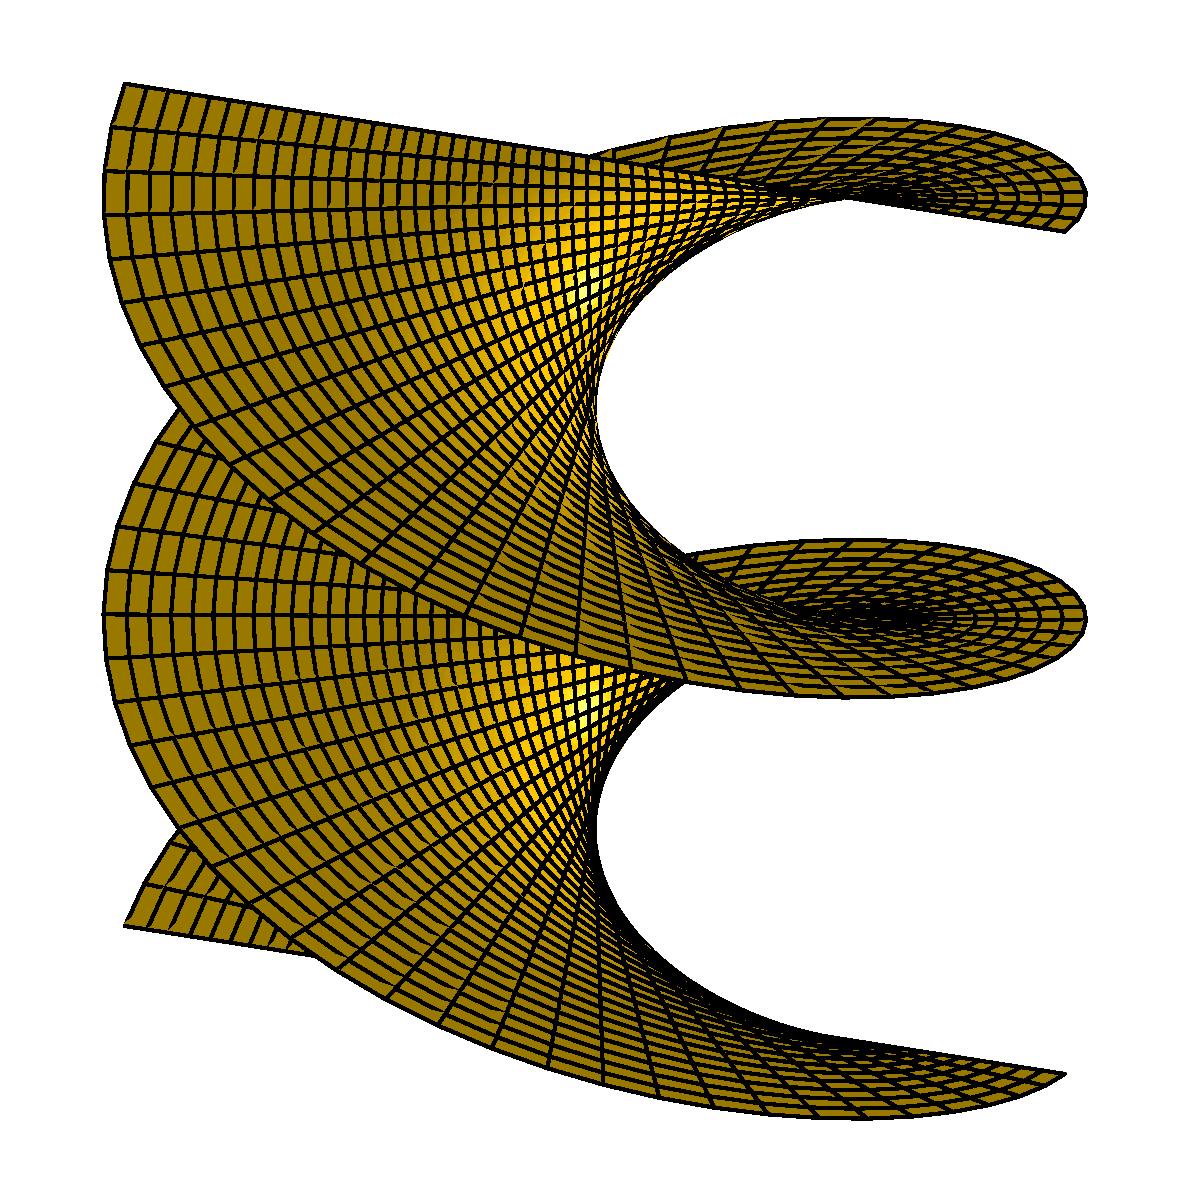
\includegraphics[width=10cm]{Images/Helicoid.eps}\end{center}


\begin{center}
Supervisors: John Bolton and Wilhelm Klingenberg
\end{center}
\end{titlepage}

\newpage
\tableofcontents
\newpage
\section{Introduction}

Believe it or not I am culminating four years of mathematics with a project about soap films - those elegant shapes that captivate the attention and imagination of every 2 year old (and for that matter a great number of adults)! Behind the beauty lie complicated mathematical problems that have been propelling forward numerous fields of mathematics since the 18th century when Jean Baptiste Meusnier (1754-1793) discovered the first examples other than the plane, in the Catenoid and Helicoid which we'll meet again later.

What makes these soap film surfaces special is that, given an arbitrarily complicated boundary, soap films minimize surface area (or in fact more generally they form at turning points of surface area). As will become apparent later all minimal surfaces satisfy the condition that they have zero mean curvature.

In the mid-nineteenth century Joseph Plateau carried out experiments accurately measuring the properties of surfaces formed on wire frames. His results led him to conjecture that every closed curve which doesn't intersect itself can be spanned by a minimal surface. The problem of finding a minimal surface for a given boundary curve became known as \emph{Plateau's Problem}.

It would appear that soap films themselves answer this question but to formulate a mathematical treatment has proved more difficult.

Lagrange was able to formulate the conditions for a minimal surface into a partial differential equation but lacked the tools to solve it in order to prove the conjecture. This has spurred on developments in partial differential equations, calculus of variation, complex analysis, and differential geometry.

A proof didn't appear for \emph{Plateau's Problem} until 1931 when Jesse \nohyphens{Douglas} and independently Tibor Rado, proved existence for a given boundary curve. This was a high point for the calculus of variations but said very little about the geometric properties of the surfaces or in fact how to find them! Therefore, as with so much in mathematics, the answers provided a wealth of new problems.

Research into minimal surfaces over the past 30 years has concentrated on the more open question of minimal surfaces which lack boundary curves. Further more armed with the power of Riemannian Geometry, has generalized them into higher dimensional minimal manifolds.

So is this entire field \emph {mathematics for the sake of mathematics} with the only connection to the real world being soap bubbles? No! Minimal surfaces have numerous real world uses. To understand why, we need to note some of the properties of these surfaces. Minimal surfaces: 
\begin{itemize}
	\item Minimize surface area.
	\item Form in soap films because their surface tension is in equilibrium at each point in the surface.
\end{itemize}

The most obvious real world example of minimal surfaces is in architecture - notably in the construction of roofs, having a minimal surface area, minimizes weight and cost of materials. Further by having surface tension in equilibrium at each point in a roof stabilizes the whole structure making it stronger. Figure \ref{fig:munich} shows a section of the roof of the Olympic Stadium in Munich the entirety of which is a minimal surface. As you can see while the properties of minimal surfaces make them ideal for such purposes they are also very aesthetically pleasing!

\begin{figure}[htbp]
	\centering
       
\includegraphics[width=8cm]{Images/Munich.eps}
   \caption{Munich Olympic Stadium \cite{MUN}}
   \label{fig:munich}
\end{figure} 


They also crop up widely in molecular engineering, crystallography and in the future, nanotechnology.
\newpage
\section{A Review of Differential Geometry}
The foundation of minimal surface theory comes from Differential Geometry so we will spend some time giving a brief overview of the key points. Further detail can be found in \cite{DoC} and \cite{EDG}.

\subsection{Gauss Map}
Given a surface M, at each point $p \in M$ there exists a tangent plane $T_pM$ and so we can define a unit normal at point $p$. Assuming M is an orientatable surface this unit normal $\mathbf N$ varies smoothly with $p$.

We can then define the Gauss Map, $G$ as a map from our surface M to the unit 2-sphere
$\mathit S^2 \subset \mathbb{R}^3$. Therefore it is the map $G:M \to \mathit S^2$ given by

\begin{displaymath}
\mathbf G(p) = \mathbf N_p =  \frac{(\mathbf X_u \times \mathbf X_v)}{|\mathbf X_u \times \mathbf X_v|}
\end{displaymath}

\subsection{First Fundamental Form}

This is a construct that allows us to measure lengths, angles and areas on a surface.

Let $\mathbf \alpha(t)= \mathbf X(u(t),v(t))$ be a curve in a surface $\mathbf X$, then its arc-length measured from a point $\alpha(t_0)$ is given by

\begin{displaymath}
\int_{t_0}^t ||\mathbf{\dot{\alpha}}(t)|| dt
\end{displaymath}

Take $\mathbf \alpha(t) = <X_1(u(t),v(t)),X_2(u(t),v(t)),X_3(u(t),v(t))>$ and using the chain rule:

\begin{eqnarray}
\nonumber
\mathbf{\dot{\alpha}}(t) &=& <\frac{\partial X_1}{\partial t},\frac{\partial X_2}{\partial t},\frac{\partial X_3}{\partial t}> \\
\nonumber
&=& <\frac{\partial X_1}{\partial u}\frac{\partial u}{\partial t}+ \frac{\partial X_1}{\partial v}\frac{\partial v}{\partial t},\frac{\partial X_2}{\partial u}\frac{\partial u}{\partial t}+ \frac{\partial X_2}{\partial v}\frac{\partial v}{\partial t},\frac{\partial X_3}{\partial u}\frac{\partial u}{\partial t}+ \frac{\partial X_3}{\partial v}\frac{\partial v}{\partial t}> \\
\nonumber
&=&\mathbf X_u \dot u+ \mathbf X_v \dot v
\end{eqnarray}

Then 
\begin{eqnarray}
\nonumber
||\mathbf{\dot{\alpha}}||^2 &=& (\mathbf X_u \dot u+ \mathbf X_v \dot v) \cdot (\mathbf X_u \dot u+ \mathbf X_v \dot v) \\
\nonumber
&=&(\mathbf X_u \cdot \mathbf X_u)\dot{u}^2 +(\mathbf X_u \cdot \mathbf X_v)\dot{u}\dot{v} + (\mathbf X_v \cdot \mathbf X_u)\dot{v}\dot{u} + (\mathbf X_v \mathbf X_v)\dot{v}^2 \\
\nonumber
&=&(\mathbf X_u \cdot \mathbf X_u)\dot{u}^2 + 2(\mathbf X_u \cdot \mathbf X_v)\dot{u}\dot{v} + (\mathbf X_v \mathbf X_v)\dot{v}^2 \\
\nonumber
&=& E\dot{u}^2 + 2F\dot{u}\dot{v} + G\dot{v}^2
\end{eqnarray}

Where we define the coefficients E, F and G as:

\begin{displaymath}
E = \mathbf X_{u} \cdot \mathbf X_u
\end{displaymath}

\begin{displaymath}
F = \mathbf X_{u} \cdot \mathbf X_v
\end{displaymath}

\begin{displaymath}
G = \mathbf X_{v} \cdot \mathbf X_v
\end{displaymath}


\subsection{Second Fundamental Form}
We take a surface S parametrised by $\mathbf x(u,v)$, a point p $\in S$ and a parametrised curve on S, $\alpha (t) = \mathbf x(u(t),v(t))$. (In order to keep the notation simple all functions that appear below denote their values at the point $p$).

Now the tangent vector to $\alpha (t)$ at p is 
\begin{displaymath}
\alpha ' = \mathbf x_u du+ \mathbf x_v dv
\end{displaymath}
and 
\begin{displaymath}
d\mathbf N(\alpha ')=\mathbf N'(u(t),v(t))=\mathbf N_udu+\mathbf N_vdv
\end{displaymath}

The second fundamental form in the basis $\{ \mathbf x_u, \mathbf x_v \}$ is given by

\begin{displaymath}
II_p = <d\mathbf N(\alpha'),\alpha'> 
\end{displaymath}

\begin{displaymath}
= -<(\mathbf N_u du + \mathbf N_v dv ) , ( \mathbf x_u du+ \mathbf x_v dv) >
\end{displaymath}

\begin{displaymath}
= -<\mathbf N_u, \mathbf x_u> du^2 - 2<\mathbf N_v, \mathbf x_u>du dv -<\mathbf N_v, \mathbf x_v> dv^2
\end{displaymath}

\begin{displaymath}
= <\mathbf N, \mathbf x_{uu}>(du)^2 + 2<\mathbf N, \mathbf x_{uv}>du dv + <\mathbf N, \mathbf x_{vv}> dv^2
\end{displaymath}

Generally we write this as

\begin{displaymath}
L du^2 + M du dv + N dv^2
\end{displaymath}

Where we define the coefficients L, M and N as:

\begin{displaymath}
L = \mathbf x_{uu} \cdot \mathbf N
\end{displaymath}

\begin{displaymath}
M = \mathbf x_{uv} \cdot \mathbf N
\end{displaymath}

\begin{displaymath}
N = \mathbf x_{vv} \cdot \mathbf N
\end{displaymath}

\subsection{Gaussian and Mean Curvature}
\label{MeanCurve}
The Gaussian and Mean Curvature, K and H measure the rate of change of the Gauss Map.

Given a surface $\mathbf{X}(u,v)$ with Guass Map $\mathbf{G}(p) = \mathbf N_p$ then

\begin{eqnarray}
\nonumber
K &=& \det(-d\mathbf N_p) = a_{11}a_{22} - a_{12}a_{21} \\
\nonumber
H &=& \frac{1}{2}\mbox{Trace}(-d\mathbf N_p) = \frac{1}{2}(a_{11}+ a_{22})
\end{eqnarray}

where 

\begin{displaymath}
d\mathbf N_p =
\left( \begin{array}{cc}
a_{11} & a_{21} \\
a_{12} & a_{22}
\end{array} \right)
\end{displaymath}

Such that
\begin{eqnarray}
\nonumber
\mathbf G_*(\mathbf x_u) &=& \mathbf N_u(p) = a_{11} \mathbf x_u + a_{21} \mathbf x_v \\
\nonumber
\mathbf G_*(\mathbf x_v) &=& \mathbf N_v(p) = a_{12} \mathbf x_u + a_{22} \mathbf x_v
\end{eqnarray}

These curvatures can also be expressed in terms of the principal curvatures of a surface. If you imagine a surface has two principal directions that span the surface (it being a 2 dimensional object) then these principal curvatures give the curvature along those curves. Taking these principal curvatures as $\kappa_1$ and $\kappa_2$ we get

\begin{displaymath}
K=\kappa_1\kappa_2
\end{displaymath}
\begin{displaymath}
H=\frac{1}{2}(\kappa_1+\kappa_2)
\end{displaymath}

The preceding definitions for Gauss and Mean curvature give the best idea of actually what the two curvatures are measuring. We will also meet $dN_p$ again later as the \emph{Weingarten Map}, A when we come to generalise minimal surfaces to higher dimensions.

We can however use Gauss's \emph{Theorema Egregium} to write these curvatures in terms of the first and second fundamental form. They are easiest to calculate in this form.

Giving

\begin{equation}
K = \frac{LN - M^2}{EG-F^2}
\label{equ:K}
\end{equation}

\begin{equation}
H = \frac{LG-2MF+NE}{2(EG-F^2)}
\label{equ:H}
\end{equation}


\newpage
\subsection{Examples}
As with much mathematics it's easiest to see the above ideas in the form of a couple of examples.
\begin{example}[Graph Type Parametrisation]
\label{Saddle}
For the saddle given by 

\begin{displaymath}
\mathbf x(u,v) = (u,v,u^2-v^2)
\end{displaymath}

\begin{figure}[htbp]
	\centering
       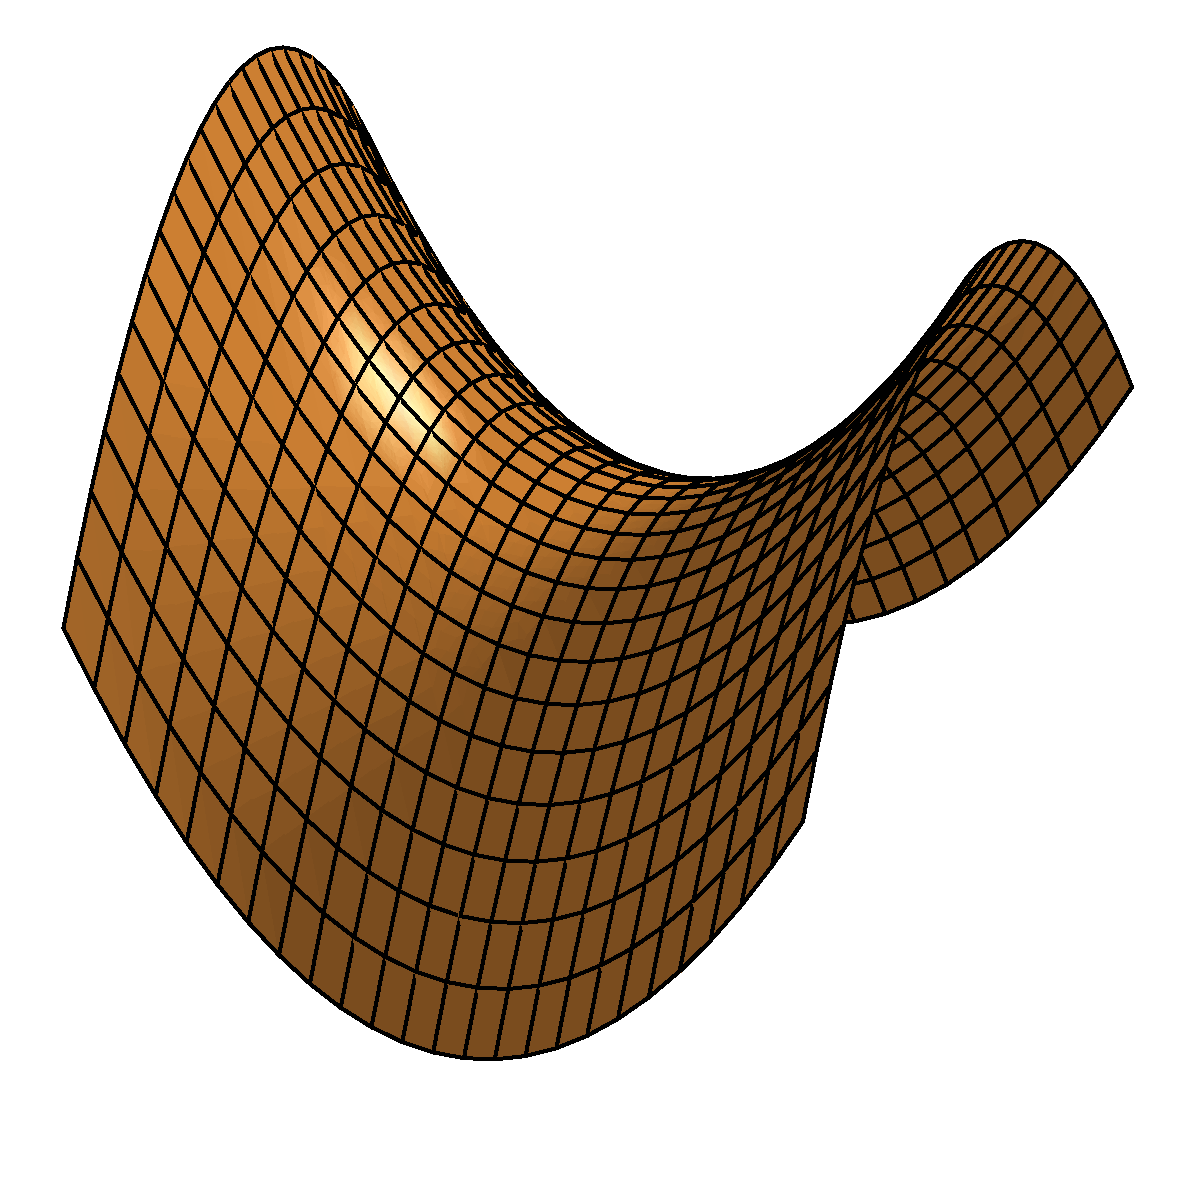
\includegraphics[width=8cm]{Images/Saddle.eps}
   \caption{Saddle}
   \label{fig:saddle}
\end{figure} 

Calculate the Gauss Map and the Second Fundamental Form. 

\begin{eqnarray}
\nonumber
\mathbf x_u &=& (1, 0 , 2u) \\
\nonumber
\mathbf x_v &=& (0, 1, -2v) \\
\nonumber
\mathbf x_{uu} &=& (0, 0 , 2) \\
\nonumber
\mathbf x_{vv} &=& (0, 0, -2) \\
\nonumber
\mathbf x_{uv} &=& (0, 0 , 0)
\end{eqnarray}

The Gauss map is then:
\begin{eqnarray}
\nonumber
G(p) = \mathbf N_p &=& \frac{(\mathbf x_u \times \mathbf x_v)}{|\mathbf x_u \times \mathbf x_v|} \\
\nonumber
&=&\frac{1}{\sqrt{1+4u^2+4v^2}}(-2u,2v,1)
\end{eqnarray}

The coefficients for the second fundamental form are:

\begin{eqnarray}
\nonumber
L &=& \mathbf x_{uu} \cdot \mathbf N = 2\,{\frac {1}{\sqrt {1+4\,{u}^{2}+4\,{v}^{2}}}}\\
\nonumber
M &=& \mathbf x_{uv} \cdot \mathbf N = 0\\
\nonumber
N &=& \mathbf x_{vv} \cdot \mathbf N = -2\,{\frac {1}{\sqrt {1+4\,{u}^{2}+4\,{v}^{2}}}}
\end{eqnarray}

So

\begin{displaymath}
II_p = ({\frac {1}{\sqrt {1+4\,{u}^{2}+4\,{v}^{2}}}})(2,0,-2)
\end{displaymath}

Then at the point p, $X(0,0)$ find the Gaussian and the Mean Curvature.

\begin{eqnarray}
\nonumber
\mathbf N_u &=& (-2,0,0) \\
\nonumber
\mathbf N_v &=& (0,2,0)
\end{eqnarray}

Projecting into the tangent plane gives

\begin{displaymath}
\mathbf N_u = -2 \mathbf x_u + 0 \mathbf x_v
\end{displaymath}

\begin{displaymath}
\mathbf N_v = 0 \mathbf x_u + 2 \mathbf x_v
\end{displaymath}

\begin{displaymath}
d\mathbf N_p =
\left( \begin{array}{cc}
-2 & 0 \\
0 & 2
\end{array} \right)
\end{displaymath}

So $ K(p) = 2 \cdot -2 = -4 $ and $H(p) = \frac{1}{2}(2 + -2) = 0$
\end{example}
\newpage

\begin{example}[Surface of Rotation]

For the surface formed by rotating $y=x^2$ about the y-axis calculate the Gauss Map and the Second Fundamental Form. 

\begin{figure}[htbp]
	\centering
       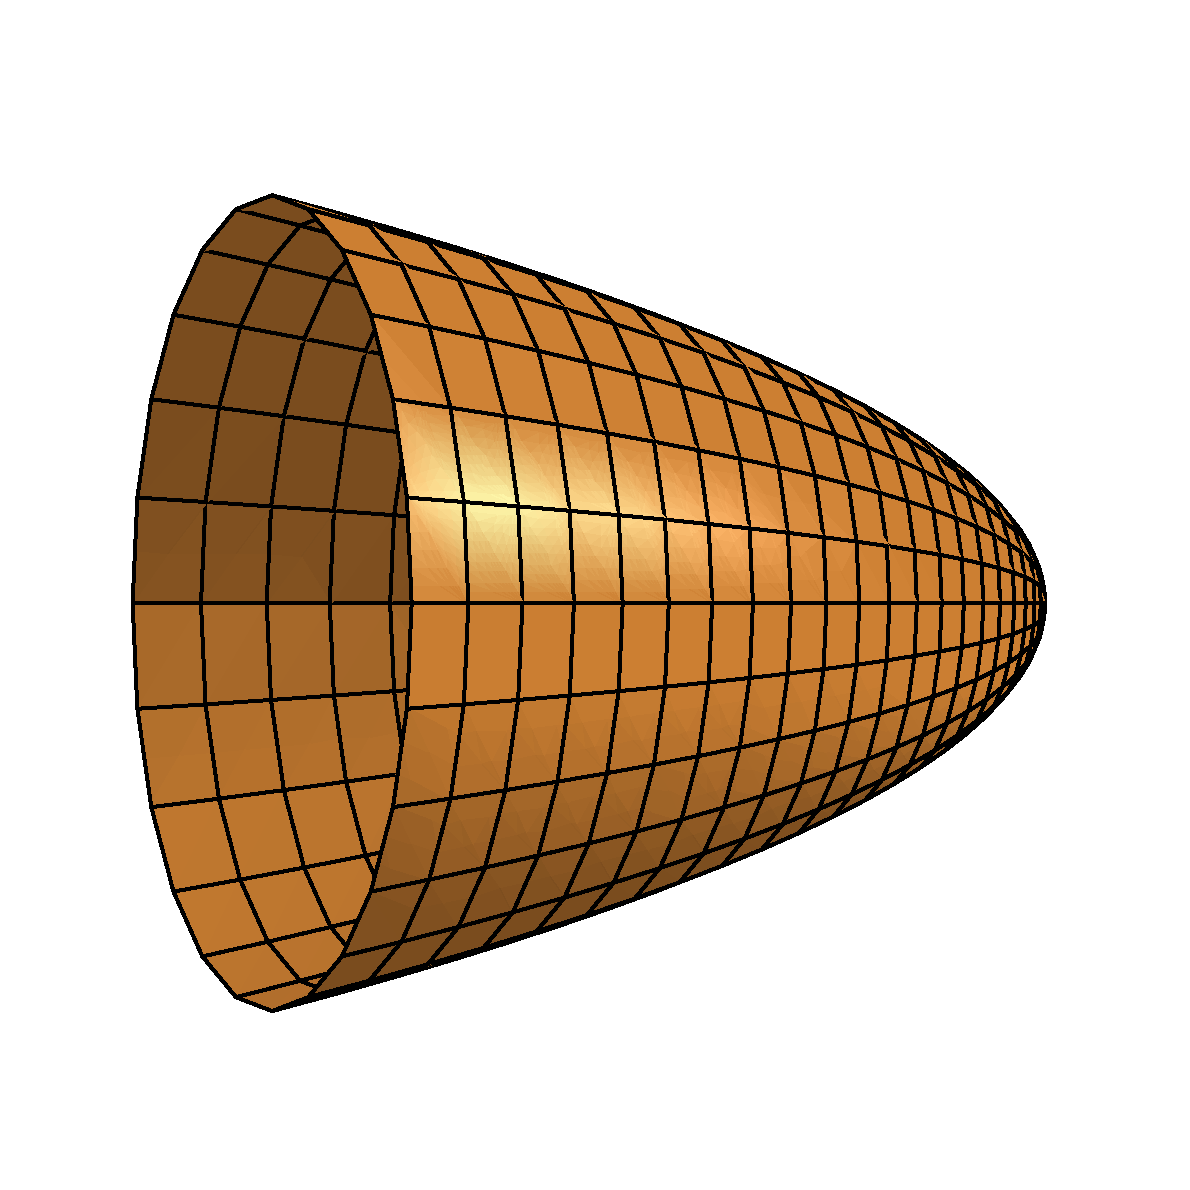
\includegraphics[width=8cm]{Images/Paraboloid.eps}
   \caption{Paraboloid}
   \label{fig:paraboloid}
\end{figure} 

Parametrised as $ \mathbf x(u,v) = (u\cos(v),u^2,u\sin(v))$

\begin{displaymath}
\mathbf x_u = (\cos v, 2u , \sin v) \, \,
\mathbf x_v = (-u \sin v, 0, u \cos v)
\end{displaymath}

\begin{displaymath}
\mathbf x_{uu} = (0, 2 , 0) \, \,
\mathbf x_{vv} = (- u \cos v, 0, - u  \sin v)
\end{displaymath}

\begin{displaymath}
\mathbf x_{uv} = (- \sin v, 0 , \cos v)
\end{displaymath}

The Gauss map is then:
\begin{eqnarray}
\nonumber
\mathbf G(p) &=& \frac{(\mathbf x_u \times \mathbf x_v)}{|\mathbf x_u \times \mathbf x_v|} \\ 
\nonumber
&=&\frac{1}{\sqrt{1+4u^2}}(2u cos v , -1 ,2u sin v)
\end{eqnarray}

The Second Fundamental Form is

\begin{displaymath}
II_p = \frac {-1}{\sqrt{1+4u^2}}(2,0, 2u^2)
\end{displaymath}

Then at the point p, $\mathbf x(\frac{1}{2},0)$ find the Gaussian and the Mean Curvature.

\begin{eqnarray}
\nonumber
\mathbf N_u &=& (\frac{1}{2}\sqrt{2},\frac{1}{2}\sqrt{2},0) = \frac{1}{2}\sqrt{2} \cdot \mathbf x_u + 0 \cdot \mathbf x_v \\
\nonumber
\mathbf N_v &=& (0,0,\frac{1}{2}\sqrt{2}) = 0 \cdot \mathbf x_u + \sqrt{2} \cdot \mathbf x_v
\end{eqnarray}

\begin{displaymath}
d\mathbf N_p =
\left( \begin{array}{cc}
\frac{1}{2}\sqrt{2} & 0 \\
0 & \sqrt{2}
\end{array} \right)
\end{displaymath}

So $ K = -\frac{1}{2}\sqrt{2} \cdot -\sqrt{2} = 1 $ and $H = \frac{1}{2}(-\frac{1}{2}\sqrt{2} - \sqrt{2}) = -\frac{3}{4}\sqrt{2}$

\end{example}

\subsection{What is a minimal surface?}
We now have enough differential geometry to define a minimal surface.

\begin{definition}[Minimal Surface]
A surface whose mean curvature, $H=0$ at all points. (E.g. note that the saddle in Example \ref{Saddle} is not minimal since although at $X(0,0)$, $H=0$ this is not the case elsewhere.)
\end{definition}

\newpage
\section{Specific Cases of Minimal Surfaces}
Having defined a minimal surface using Differential Geometry, we now ask what minimal surfaces actually exist and how do we find them? We will start by setting up a partial differential equation known as the minimal surface equation. However it will quickly become apparent that a general solution of this equation is not possible, we will therefore impose various geometric and algebraic constraints which will then allow us to solve for different classes of minimal surfaces.

\subsection{The Minimal Surface Equation}
Locally all surfaces can be defined by a Monge parametrisation  $z= f(x,y)$ so

\begin{displaymath}
\mathbf x(u,v) = (x, y, f(x,y))
\end{displaymath}

Calculating the first and second fundamental forms gives:

\begin{displaymath}
E = 1 + f_x^2 \ \ F = f_xf_y \ \ G = 1+f_y^2
\end{displaymath}

\begin{displaymath}
L = \frac{f_{xx}}{\sqrt{1+f_x^2+f_y^2}} \ \ M = \frac{f_{xy}}{\sqrt{1+f_x^2+f_y^2}} \ \ N = \frac{f_{yy}}{\sqrt{1+f_x^2+f_y^2}}
\end{displaymath}

Subbing these into our equation for Mean Curvature (Equation \ref{equ:H}) and equating to zero gives:
\begin{equation}
\framebox{$f_{xx}(1+f_y^2)-2f_{xy}f_xf_y+f_{yy}(1+f_x^2)=0$}
\label{equ:MinimalSurfaceEquation}
\end{equation}
Unfortunately in general this is not solvable by simple means. If we look for a surface defined globally we discover that the only such minimal surface is the plane, this is known as Bernstein's Theorem.
\begin{theorem}[Bernstein]
If a minimal surface $M: \, z=f(u,v)$ is defined on the whole xy-plane, then M is a plane.
\end{theorem}

However locally there are many such minimal surfaces, one of the most famous of these is \emph{Scherk's First Surface}.

\subsection{Scherk's First Surface}
We've already derived the minimal surface equation and said that it is not solvable by simple means however; we will apply an algebraic condition which will make the equation solvable.

We will look for surfaces with $f(x,y) = g(x) + h(y)$. Such surfaces are known as translation surfaces but we are interested in them because it allows us to separate variables leaving us with two ordinary differential equations which we can solve.

Letting $\mathbf x(x,y) = (x, y, g(x) + h(y))$ and following the same procedure as for the \emph{Minimal Surface Equation} (or in fact subbing $f(x,y) = g(x) + h(y)$ directly into equation \ref{equ:MinimalSurfaceEquation}). This gives us

\begin{equation}
g_{xx}(x)(1+h_y^2(y))+h_{yy}(y)(1+g_x^2(x)) = 0 
\label{equ:ScherkMinSurf}
\end{equation}

Rearranging gives

\begin{displaymath}
-\frac{1+g_x^2(x)}{g_{xx}(x)} = \frac{1+h_y^2(y)}{h_{yy}(y)}
\end{displaymath}

Now note that the LHS is a function of only x and the RHS is a function of only y. Varying one of these and holding the other fixed therefore cannot change anything, e.g. both sides are equal to the same constant.

\begin{displaymath}
-\frac{1+g_x^2(x)}{g_{xx}(x)} = c = \frac{1+h_y^2(y)}{h_{yy}(y)}
\end{displaymath}

This gives us two ordinary differential equations which we can then solve to find $g(x)$ and $h(y)$.

\begin{eqnarray}
\label{equ:Scherk_g}
1+g_x^2(x) &=& - cg_{xx}(x) \\
\label{equ:Scherk_h}
1+h_y^2(y) &=& ch_{yy}(y)
\end{eqnarray}

Both of these equation solve in exactly the same way (obviously noting the minus sign in \ref{equ:Scherk_g}). We will therefore just solve \ref{equ:Scherk_g} and state the result for \ref{equ:Scherk_h}.

Equation \ref{equ:Scherk_g} has no dependence on g(x), so we can set $\phi = g_x(x)$ which gives us

\begin{displaymath}
1+\phi^2 = -c\phi_x
\end{displaymath}

We can now separate and integrate:
\begin{displaymath}
\int\frac{-c}{1+\phi^2}d\phi = \int dx
\end{displaymath}

Letting $\phi = \tan \theta$ giving $\frac{d\phi}{d\theta} = \sec^2\theta$ and subbing in:

\begin{eqnarray}
\nonumber
\int\frac{-c}{1+\tan^2\theta}\sec^2\theta d\theta &=& \int dx \\
\nonumber
\Leftrightarrow \int\frac{-c}{\sec^2\theta}\sec^2\theta d\theta &=& \int dx \\
\nonumber
\Leftrightarrow \int\frac{-c}{\sec^2\theta}\sec^2\theta d\theta &=& \int dx \\
\nonumber
\Leftrightarrow -c\int d\theta &=& \int dx \\
\nonumber
\Leftrightarrow -c\theta &=& x \mbox{\ \ \ \ supressing constant of integration} \\
\nonumber
\Leftrightarrow -c \arctan \phi &=& x \\
\nonumber
\therefore \phi &=& -\tan\left(\frac{x}{c}\right)
\end{eqnarray}

Now re-writing in terms of g(x) gives:

\begin{displaymath}
g_x(x) = -\tan\left(\frac{x}{c}\right)
\end{displaymath}

Integrating this up gives

\begin{displaymath}
g(x) = c \ln\left((\cos \left(\frac{x}{c}\right)\right)
\end{displaymath}

Following this method exactly but taking the change of sign into account for equation \ref{equ:Scherk_h} gives

\begin{displaymath}
h(y) = -c \ln\left(\cos \left(\frac{y}{c}\right)\right)
\end{displaymath}
 
Putting these back together we get our $f(x,y)$.

\begin{eqnarray}
\nonumber
f(x,y) &=& g(x) + h(y) \\
\nonumber
&=& c \ln(\cos \left(\frac{x}{c}\right))-c \ln(\cos \left(\frac{y}{c}\right)) \\
\label{equ:Scherk_f}
&=& c \ln\left(\frac{cos(x/c)}{cos(y/c)}\right)
\end{eqnarray}

The surface $z=f(x,y)$ is known as \emph{Scherk's (first) minimal surface}. Since the logarithm function is only defined for positive values, Scherk's surface is only defined for $\frac{cos(x/c)}{cos(y/c)} > 0$. Therefore, for example letting $c=1$, Scherk's surface forms a chess board pattern with the surface defined on squares with vertices at points $\left(\frac{\pi}{2}+m\pi,\frac{\pi}{2}+n\pi\right)$, where m and n are integers. This can be seen in Figure \ref{fig:scherk}.

\begin{figure}[htbp]
	\centering
       \includegraphics[width=8cm]{Images/Scherk.eps}
   \caption{Scherk's First Minimal Surface}
   \label{fig:scherk}
\end{figure} 

\subsection{Surfaces of Revolution}
We have just seen what happens when we impose an algebraic condition on the minimal surface equation; however we can also impose geometric conditions in order to find minimal surfaces. We will now find all surfaces of revolution which are minimal. 
\begin{definition}[Surface of Revolution]
A surface of revolution is defined by rotating a plane curve around a straight line in the plane. They are surfaces of the form
\begin{displaymath}
\mathbf x(u,v) = (f(v) \cos(u), f(v) \sin(u), v)
\end{displaymath}
\end{definition}

We start as normal by calculating the coefficients of the first and second fundamental forms from which we will set up an equation for Mean Curvature. Setting this to zero will give us an ordinary differential equation whose solutions are the only minimal surfaces of revolution.

\begin{eqnarray}
\nonumber
E &=& \mathbf x_u \cdot \mathbf x_u = f(v)^2 \\
\nonumber
F &=& \mathbf x_u \cdot \mathbf x_v = 0 \\
\nonumber
G &=& \mathbf x_v \cdot \mathbf x_v = 1 + f'(v)^2
\end{eqnarray}

\begin{eqnarray}
\nonumber
L &=& \mathbf x_{uu} \cdot \mathbf N = -\frac{f(v)}{\sqrt{1+f'(v)^2}} \\
\nonumber
M &=& \mathbf x_{uv} \cdot \mathbf N = 0 \\
\nonumber
N &=& \mathbf x_{vv} \cdot \mathbf N = \frac{f''(v)}{\sqrt{1+f'(v)^2}}
\end{eqnarray}

Now using the standard result that $H=\frac{1}{2} \frac{LG-2MF+NE}{EG-F^2}$, which for a minimal surface equals zero.

Gives

\begin{eqnarray}
\nonumber
H = -\frac{1}{2} \frac{1+f'(v)^2-f(v) f''(v)}{f(v)(1+f'(v)^2)^{\frac{3}{2}}} &=& 0 \\
\nonumber
\Leftrightarrow \frac{1+(f')^2-ff''}{f(1+(f')^2)^{\frac{3}{2}}} &=& 0 \\
\nonumber
\Leftrightarrow \frac{1}{f\sqrt{(1+(f')^2)} }-\frac{ff''}{(1+(f')^2)^{\frac{3}{2}}} &=& 0 \\
\nonumber
\Leftrightarrow \frac{1}{f}&=&\frac{f''}{1+(f')^2} \\
\nonumber
\times 2f' \ \ \ \ \ \Leftrightarrow \frac{2f'}{f}&=&\frac{2f'f''}{1+(f')^2}
\end{eqnarray}

Subbing in $1+(f')^2 = z$ $\Leftrightarrow$ $z' = 2y'y''$ gives

\begin{displaymath}
\frac{2f'}{f}=\frac{z'}{z}
\end{displaymath}

and integrating:

\begin{displaymath}
2\ln(f)+\ln(k) = \ln(z) \mbox{\ \ \ Where k in a constant of integration}
\end{displaymath}

\begin{eqnarray}
\nonumber
\Leftrightarrow \ln(fk)^2 &=& \ln(z) \\
\nonumber
\Leftrightarrow 1+(f')^2 &=& (fk)^2 \\
\nonumber
\Leftrightarrow \frac{f'}{\sqrt{(fk)^2-1}} &=& 1
\end{eqnarray}

\begin{eqnarray}
\nonumber
\times k \mbox{ and integrate:} \ \ \ \ \int \frac{k}{\sqrt{(fk)^2-1}} df &=& \int k dv \\
\nonumber
\Leftrightarrow \cosh^{-1}(fk) &=& kv + c \\
\nonumber
\therefore f(v) &=& \frac{1}{k} \cosh(kv+c)
\end{eqnarray}

We only have a single solution, therefore the only minimal surface of revolution is $\mathbf x(u,v) = (\frac{1}{k} \cosh(kv+c) cos(u), \frac{1}{k} \cosh(kv+c) \sin(u), v)$ which is known as a Catenoid. Taking k = 1 results in Figure \ref{fig:catenoid}.

\begin{figure}[htbp]
	\centering
       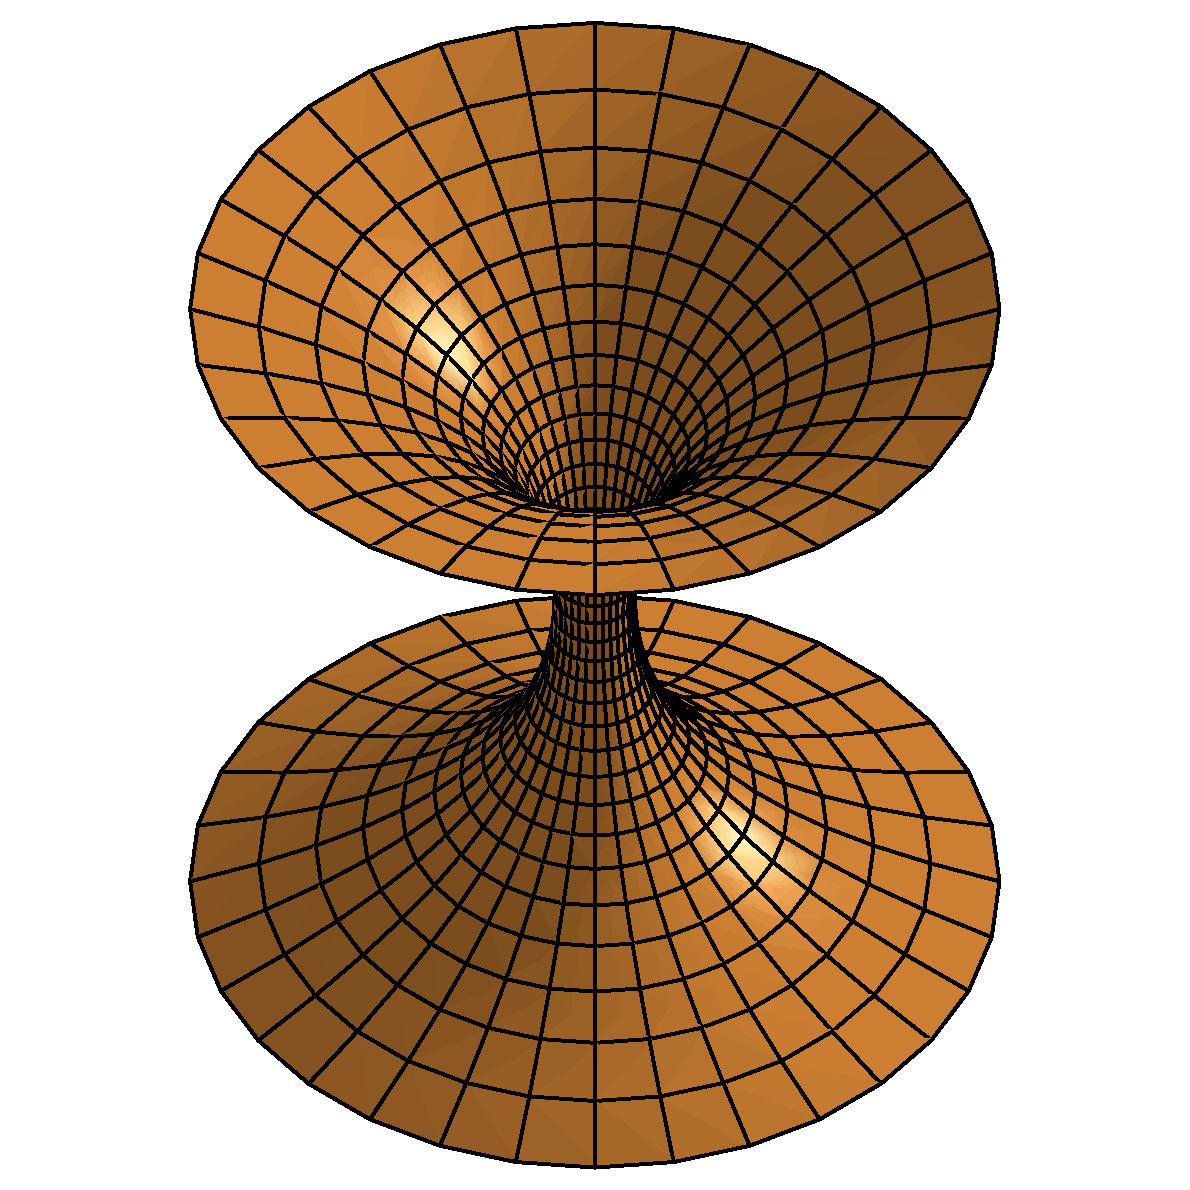
\includegraphics[width=8cm]{Images/Catenoid.eps}
   \caption{The Catenoid}
   \label{fig:catenoid}
\end{figure} 

\subsection{Ruled Surfaces}
We now apply another geometric constraint, asking that the surface be ruled.
\begin{definition}
A ruled surface is a surface parametrised by
\begin{displaymath}
\mathbf x(u,v) = \beta(u) + v \gamma(u)
\end{displaymath}

Such that we have straight lines starting on the curve $\beta(u)$ going in the direction $\gamma(u)$.
\end{definition}

There are many examples of ruled surfaces and the above definition becomes immediately obvious having seen a few.

\begin{example}[The Plane]
\begin{displaymath}
\mathbf x(u,v) =  \left[ \begin{array}{c} u\\0\\0 \end{array} \right] + v\left[ \begin{array}{c} 0\\1\\0 \end{array} \right] = \left[ \begin{array}{c} u\\v\\0 \end{array} \right]
\end{displaymath}

The plane in fact has two rulings as can be seen in figure \ref{fig:plane}. Also since it is flat it is also a minimal surface.

\begin{figure}[htbp]
	\centering
       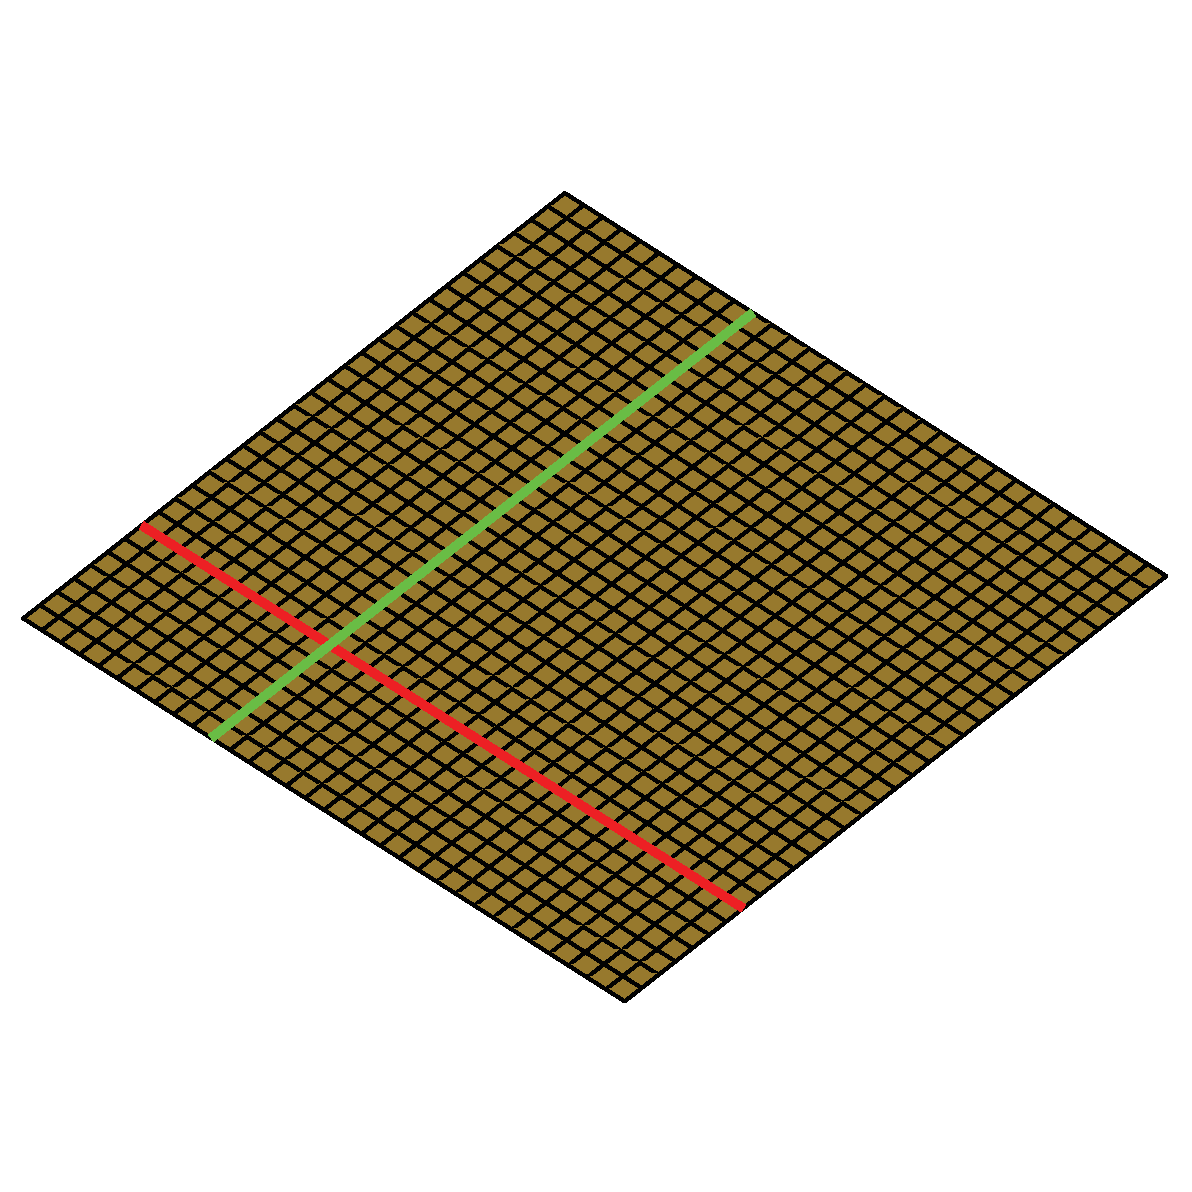
\includegraphics[width=8cm]{Images/Plane.eps}
   \caption{The Plane}
   \label{fig:plane}
\end{figure} 
\end{example}

\begin{example}[The Cone]
\begin{displaymath}
\mathbf x(u,v) =  \left[ \begin{array}{c} 0\\0\\0 \end{array} \right] + v\left[ \begin{array}{c} 1\\ \cos u \\ \sin u \end{array} \right] = \left[ \begin{array}{c} v\\v \cos u \\v \sin u \end{array} \right]
\end{displaymath}

See Figure \ref{fig:cone}.

\begin{figure}[htbp]
	\centering
       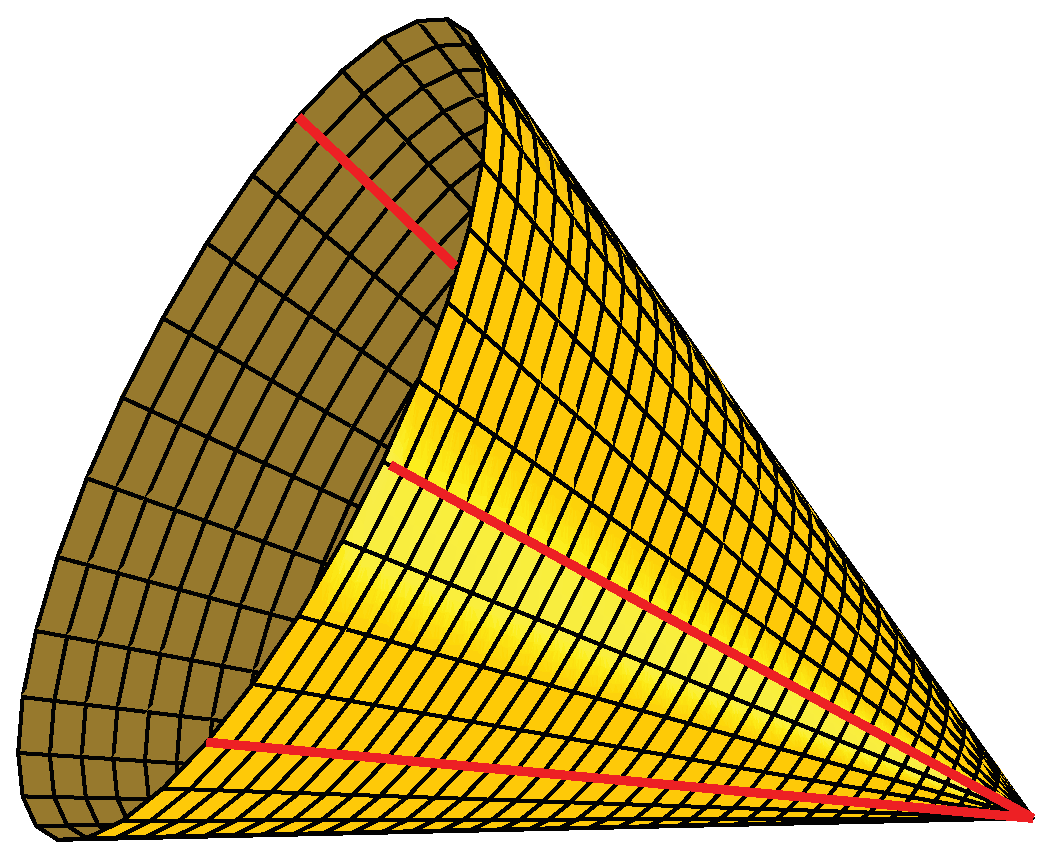
\includegraphics[width=8cm]{Images/Cone.eps}
   \caption{The Cone}
   \label{fig:cone}
\end{figure} 
\end{example}

\begin{example}[The Helicoid]
\begin{displaymath}
\mathbf x(u,v) = (a\:\sinh \: v\: cos \: u, a \: \sinh \:v \: \sin \:u, au)
\end{displaymath}

See Figure \ref{fig:helicoid}

\begin{figure}[htbp]
	\centering
       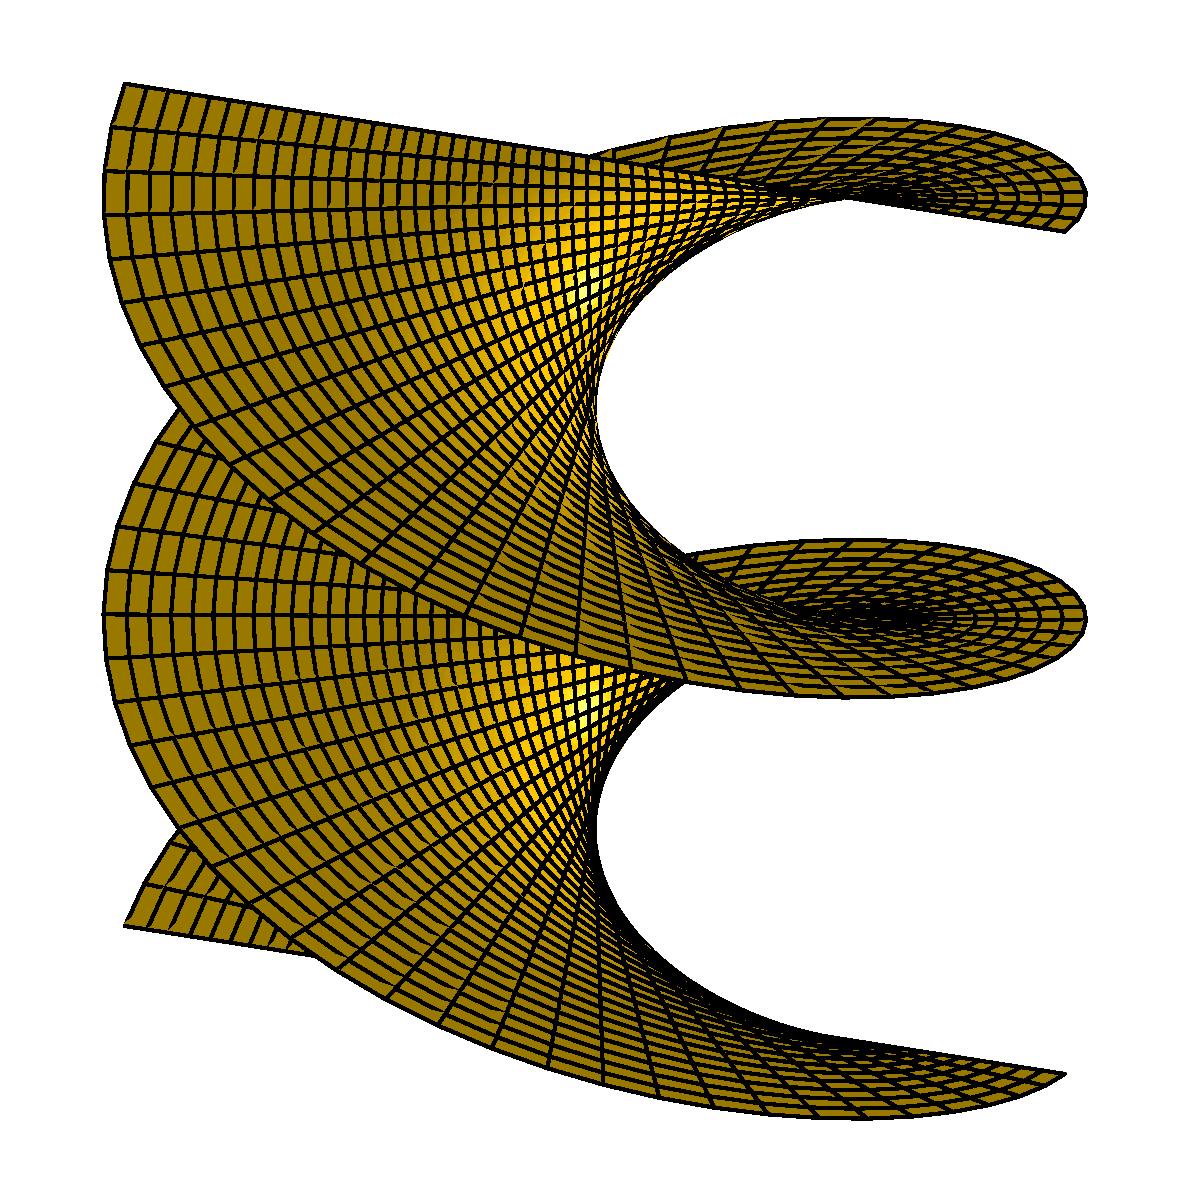
\includegraphics[width=8cm]{Images/Helicoid.eps}
   \caption{The Helicoid}
   \label{fig:helicoid}
\end{figure} 

Calculating as before $E=G= a^2cosh^2v$, $F = 0$, $L = M = 0$, $N = a^2$ gives $H=0$. So the Helicoid is a Minimal Surface.
\end{example}

\begin{theorem}
\label{Ruled}
The Helicoid is the only ruled minimal surface, other than the plane.
\label{RuledMinimal}
\end{theorem}
The proof of this requires the following:

\begin{lemma}
The zeros of the Gaussian curvature of a minimal surface are isolated.
\end{lemma}

\begin{definition}[Asymptotic Curve]
Let p be a point in S. An asymptotic direction of S at p is a direction of $T_p(S)$ for which the normal curvature is zero. An asymptotic curve of S is a regular connected curve $C \subset S$ such that for each $p \in C$ the tangent line of C at p is an asymptotic direction.
\end{definition}

\begin{definition}[Osculating Plane]
The plane determined by the unit tangent and normal vectors to a space curve as seen in figure \ref{fig:oscplane}.
\begin{figure}[htbp]
	\centering
       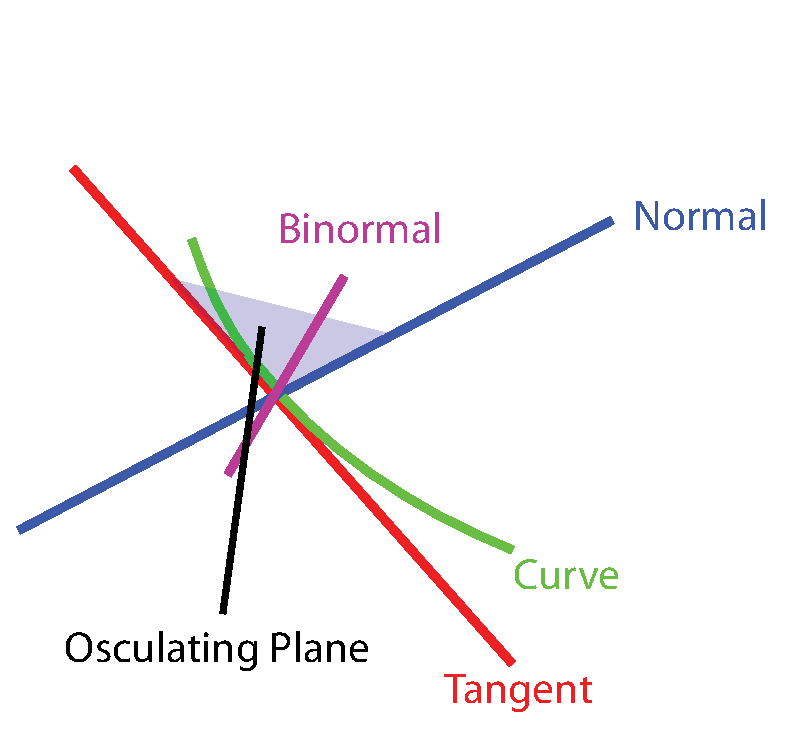
\includegraphics[width=8cm]{Images/OsculatingPlane.eps}
   \caption{Osculating Plane}
   \label{fig:oscplane}
\end{figure}
\end{definition}

\begin{definition}[Torsion]
This is the rate of change of the Osculating Plane as you move along the curve.
\end{definition}

\begin{definition}[Bertrand Curve]
let $\alpha: I \rightarrow R^3$ be a parametrised regular curve with $k(t) \neq 0$, $\tau \neq 0$, $t \in I$. The curve $\alpha$ is called a Bertrand curve if there exists a curve $\overline{\alpha}: I \rightarrow R^3$ such that the normal lines of $\alpha$ and $\overline{\alpha}$ at $t \in I$ are equal. In this case, $\overline{\alpha}$ is called a Bertrand mate of $\alpha$, and we can write

\begin{displaymath}
\overline{\alpha}= \alpha(t) + rn(t)
\end{displaymath}

\end{definition}

\begin{lemma}
If $\alpha$ has more than one Bertrand mate, it has infinitely many Bertrand mates. This case occurs if and only if $\alpha$ is a circular helix.
\label{lem:CircHelix}
\end{lemma}

\begin{proof}{Theorem \ref{RuledMinimal}}. 

Let S be a minimal ruled surface, $H=0$ and assume S is not a plane.

In some region W of S the Gaussian curvature K is strictly negative.

\begin{displaymath}
H =\frac{1}{2} (\kappa_1+\kappa_2) = 0 \Leftrightarrow \kappa_1 = -\kappa_2
\end{displaymath}

\begin{displaymath}
\Leftrightarrow K=\kappa_1 \cdot \kappa_2 < 0
\end{displaymath}

Given that S is minimal, $H=0$ and therefore W is covered by two families of asymptotic curves which intersect orthogonally. 

Since the rulings are asymptotic curves and the surface is not a plane, we can choose a point $q \in W$ such that the asymptotic curve, other than the ruling, passing though q has nonzero torsion at q.

Since the osculating plane of an asymptotic curve is the tangent plane to the surface, there exists a region in $W$ such that the rulings in this region are principal normals to the family of twisted asymptotic curves.

Lemma \ref{lem:CircHelix} says that this occurs if and only if the twisted curves are circular helices.

Therefore this region is a part of a Helicoid.

Since the torsion of a circular helix is constant, it can be seen that the whole surface is part of a Helicoid, as we claimed.
\end{proof}



\newpage
\section{Review of Complex Analysis}
The examples of minimal surfaces given previously pretty much cover the early developments in minimal surface theory. However the sheer lack of them was proving to be a bottleneck to their study. What was needed was a new way of attacking them and generating new ones. The answer came in the form of Complex Analysis.

In order to proceed we will very briefly give an overview of the main aspects of complex analysis we will be using. Further material on this subject is available in \cite{BCA}.

\subsection{The Cauchy-Riemann Equations}
These lie at the heart of complex analysis and allow us to differentiate complex functions.

The differential of a complex function is calculated using the same limit as for a real function:
\begin{displaymath}
\lim_{z\rightarrow z_0}\frac{f(z_0)-f(z)}{z-z_0}
\end{displaymath}
However we can let $z$ approach $z_0$ in any way we please. If
\begin{displaymath}
z_o = x_0 + i y_0
\end{displaymath}
we can then let $z = x_0 + h + i y_0$ or $z = x_0 + i (y_0+k)$ with $h$ and $k$ real.

However $f'(z)$ must be uniquely defined no matter how we let $z$ approach $z_0$ and so evaluating the limits of the two above cases we get

\begin{displaymath}
f'(z_0) = \frac{\partial u}{\partial x} + i \frac{\partial v}{\partial x} = \frac{\partial v}{\partial y} - i \frac{\partial u}{\partial y}
\label{CR}
\end{displaymath}
Comparing real and imaginary parts, we find that

\begin{displaymath}
\frac{\partial u}{\partial x} = \frac{\partial v}{\partial y} \ \ \  \frac{\partial v}{\partial x} =  -\frac{\partial u}{\partial y}
\end{displaymath}

These are the Cauchy-Riemann equations which hold for differentiable complex functions.

\subsection{Harmonic Functions}
Harmonic functions uncover a beautiful aspect of minimal surfaces, showing that they come in families.

Given a real valued function $\phi(x,y)$ we say that $\phi$ is a harmonic function if it satisfies \emph{Laplaces Equation}

\begin{displaymath}
\frac{\partial^2 \phi}{\partial x^2} + \frac{\partial^2 \phi}{\partial y^2} = 0 
\end{displaymath}

If $f$ is an analytic function (complex differentiable) defined in a domain $D$ and $f(z) = u(x,y)+iv(x,y)$, then we can show both u and v are harmonic in D. 

We know

\begin{displaymath}
f'(z) = \frac{\partial u}{\partial x} + i \frac{\partial v}{\partial x} = \frac{\partial v}{\partial y} - i \frac{\partial u}{\partial y}
\end{displaymath}

Setting $f' = U +iV$ and using the Cauchy-Riemann equations for U, V the partial derivatives of U and V exist and satisfy:

\begin{equation}
\frac{\partial U}{\partial x} = \frac{\partial V}{\partial y}
\label{CR_A}
\end{equation}
\begin{equation}
\frac{\partial V}{\partial x} =  -\frac{\partial U}{\partial y}
\label{CR_B}
\end{equation}

Since

\begin{displaymath}
U = \frac{\partial u}{\partial x} = \frac{\partial v}{\partial y}\ \ \  V = \frac{\partial v}{\partial x} = -\frac{\partial u}{\partial y}
\end{displaymath}

Subbing into \ref{CR_A} gives 

\begin{displaymath}
\frac{\partial}{\partial x}(\frac{\partial u}{\partial x}) 
= \frac{\partial}{\partial x}(\frac{\partial v}{\partial y})
= \frac{\partial}{\partial y}(\frac{\partial v}{\partial x})
= -\frac{\partial}{\partial y}(\frac{\partial u}{\partial y})
\end{displaymath}

So 

\begin{displaymath}
\frac{\partial^2 u}{\partial x^2} + \frac{\partial^2 u}{\partial y^2} = 0
\end{displaymath}

Subbing into \ref{CR_B} gives 

\begin{displaymath}
\frac{\partial}{\partial x}(\frac{\partial v}{\partial x}) 
= -\frac{\partial}{\partial x}(\frac{\partial u}{\partial y})
= -\frac{\partial}{\partial y}(\frac{\partial u}{\partial x})
= -\frac{\partial}{\partial y}(\frac{\partial v}{\partial y})
\end{displaymath}

So 

\begin{displaymath}
\frac{\partial^2 v}{\partial x^2} + \frac{\partial^2 v}{\partial y^2} = 0
\end{displaymath}

So if $f$ is an analytic function then its real and imaginary parts are harmonic functions.
\newpage
\section{Weierstrass-Enneper Representations}

Having laid the foundations of the complex analysis required, we can now proceed and show how to use these new tools to explore minimal surfaces. We will first introduce isothermal parameters on a minimal surface, show the connection between minimal surfaces and harmonic functions and finally come to Weierstrass-Enneper Representations which is the powerful tool that will allow us to create minimal surfaces with ease.

\subsection{Isothermal Parameters}
\begin{definition}
A parametrisation $\mathbf x(u,v)$ is isothermal if the coefficients of the first fundamental form are of the form:
\begin{displaymath}
E = G, \ \ F = 0
\label{defisothermal}
\end{displaymath}

Geometrically this means angles in the plane look exactly the same as angles on a surface with a isothermal parametrisation. We call this angle preserving.
\end{definition}

\begin{theorem}
Isothermal coordinates exist on all surfaces.
\label{isothermal}
\end{theorem}

We will only prove the case for minimal surfaces as this is all we require. 
\begin{proof}
\cite{OSS}
Fix a point $m \in M$. Choose a coordinate system for $\mathbb R^3$ so that $m$ is the origin, the tangent plane to $M$, $T_mM$, is the $xy$-plane, and near $m$, $M$ is the graph of a function $z=f(x,y)$. Furthermore, the quotient and chain rules give

\begin{displaymath}
\left(\frac{1+f_x^2}{w}\right)_y-\left(\frac{f_xf_y}{w}\right)x = -\frac{f_y}{w}\left[f_{xx}(1+f^2_y)-2f_xf_yf_{xy}+f_{yy}(1+f^2_x)\right]
\end{displaymath}

\begin{displaymath}
\left(\frac{1+f_y^2}{w}\right)_x-\left(\frac{f_xf_y}{w}\right)y = -\frac{f_x}{w}\left[f_{xx}(1+f^2_y)-2f_xf_yf_{xy}+f_{yy}(1+f^2_x)\right]
\end{displaymath}

where $w=\sqrt{1+f_x^2+f_y^2}$. Let $p=f_x$, $q=f_y$ with $w^2 = 1 + p^2 + q^2$. Because $M$ is minimal, $f$ satisfies the \emph{Minimal Surface Equation}

\begin{displaymath}
f_{xx}(1+f_y^2)-2f_xf_yf_{xy}+f_{yy}(1+f_x^2)=0,
\end{displaymath}

so we have $\left(\frac{1+p^2}{w}\right)_y - \left(\frac{pq}{w}\right)_x = 0$ and $\left(\frac{1+q^2}{w}\right)_x - \left(\frac{pq}{w}\right)_y = 0$. Define two vector fields in the $xy$-plane by
\begin{displaymath}
V=\left(\frac{1+p^2}{w},\frac{pq}{w}\right) \mbox{\ \ \ \ and \ \ \ \ } W=\left(\frac{pq}{w},\frac{1+q^2}{w}\right)
\end{displaymath}
and apply Green's theorem to any closed curve C contained in a simply connected region $\it{R}$ to obtain

\begin{displaymath}
\int_C V\cdot dr = \int \int_{\it{R}}\left(\frac{pq}{w}\right)_x-\left(\frac{1+p^2}{w}\right)_y dxdy=0,
\end{displaymath}

\begin{displaymath}
\int_C W\cdot dr = \int \int_{\it{R}}\left(\frac{1+q^2}{w}\right)_x - \left(\frac{pq}{w}\right)_y dxdy=0,
\end{displaymath}

where $dr = (dx,dy)$. Since the line integrals are zero for all closed curves in $\it R$, $V$ and $W$ must have potential functions (see \cite{MT}). That is, there exist $\mu$ and $\rho$  with $\mbox{grad }(\mu)= V$ and $\mbox{grad }(\rho) = W$. Considered coordinatewise, these equations imply $\mu_x = \frac{1+p^2}{w}$, $\mu_y=\frac{pq}{w}$ and $\rho_x = \frac{pq}{w}$, $\rho_y = \frac{1+q^2}{w}$. Define a mapping $T:\it R \rightarrow \mathbb R^2$ by

\begin{displaymath}
T(x,y) = (x+\mu(x,y),y+\rho(x,y)).
\end{displaymath}

The Jacobian matrix of this mapping is then
\begin{displaymath}
J(T)= \left[ \begin{array}{cc}
1+\mu_x & \rho_y \\
\rho_x & 1+\rho_y
\end{array} \right] = \left[ \begin{array}{cc}
1+\frac{1+p^2}{w} & \frac{pq}{w} \\
\frac{pq}{w} & 1+ \frac{1+q^2}{w}
\end{array} \right],
\end{displaymath}

and we calculate the determinant to be $det(J(T)) = \frac{(1+w)^2}{w} > 0$. The Inverse Function Theorem then says that, near $m=(0,0)$, there is a smooth inverse function $T^{-1}(u,v)=(x,y)$ with

\begin{eqnarray}
\nonumber
J(T^{-1})&=&J(T)^{-1} \\
\nonumber
&=&\frac{1}{\mbox{det }J(T)}\left[ \begin{array}{cc}
1+\frac{1+p^2}{w} & \frac{pq}{w} \\
\frac{pq}{w} & 1+ \frac{1+q^2}{w}
\end{array} \right] \\
\nonumber
&=&\frac{1}{(1+w)^2}\left[ \begin{array}{cc}
w+1+q^2 & pq \\
-pq & 1+ w+1+p^2
\end{array} \right]
\end{eqnarray}

Of course, for $(x,y) = T^{-1}(u,v)$, the last matrix is just
\begin{displaymath}
\left[ \begin{array}{cc}
x_u & x_v \\
y_u & y_v
\end{array} \right]
\end{displaymath}
by the definition of the Jacobian. We will put these calculations to use in showing that the parametrisation (in the $u,v$ coordinates described above) $\mathbf x(u,v) \stackrel{def}{=}(x(u,v),\ y(u,v),\ f(x(u,v),y(u,v)))$ is isothermal.

First calculate

\begin{eqnarray}
\nonumber
\mathbf x_u &=& \left(\frac{w+1+q^2}{(1+w)^2},\frac{-pq}{(1+w)^2},p\left(\frac{w+1+q^2}{(1+w)^2}\right)+q\left(\frac{-pq}{(1+w)^2}\right)\right) \\
\nonumber
\mathbf x_u &=& \left(\frac{-pq}{(1+w)^2},\frac{w+1+p^2}{(1+w)^2},p\left(\frac{(-pq)(w+1+q^2)}{(1+w)^2}\right)+q\left(\frac{w+1+p^2}{(1+w)^2}\right)\right)
\end{eqnarray}

Now all that remains is to calculate the coefficients of the first fundamental form:

\begin{eqnarray}
\nonumber
E &=& \mathbf x_u \cdot \mathbf x_u \\
\nonumber
&=& \frac{1}{(1+w)^4}[(w+1+q^2)^2 + p^2q^2 +p^2(w+1+q^2)^2 \\
\nonumber
&\ & \ \ \ \ -2p^2q^2(w+1+q^2)+p^2q^4]\\
\nonumber
&=& \frac{1}{(1+w)^4}[(1+w)^2(1+q^2+p^2)] \\
\nonumber
&=& \frac{w^2}{(1+w)^2} \\
\nonumber
G &=& \mathbf x_v \cdot \mathbf x_v \\
\nonumber
&=&\frac{1}{(1+w)^4}[p^2q^2+(w+1+p^2)^2+ p^4q^2 \\
\nonumber
&\ & \ \ \ \ -2q(w+1+p^2)p^2q+q(w+1+p^2)^2] \\
\nonumber
&=&\frac{1}{(1+w)^4}[(1+w)^2(1+q^2+p^2)] \\
\nonumber
&=&\frac{w^2}{(1+w)^2} \\
\nonumber
&=& E
\end{eqnarray}
\begin{eqnarray}
\nonumber
F &=& \mathbf x_u \cdot \mathbf x_v \\
\nonumber
&=&\frac{1}{(1+w)^4}[-(w+1+q^2)pq - pq(w+1+p^2) \\
\nonumber
&\ & \ \ \ \ + (p(w+1+q^2)-q^2p)(-p^2q+q(w+1+p^2))] \\
\nonumber
&=&\frac{1}{(1+w)^4}[-\cancel{pqw}-\cancel{pq}-pq^3-\cancel{pqw}-pq-p^3q+pw^2q+\cancel{2pqw}+\cancel{pq} \\
\nonumber
&=&-pq^3-pq-p^3q+pw^2q \\
\nonumber
&=&-pq^3-pq-p^3q+pq(1+p^2+q^2) \\
\nonumber
&=& 0
\end{eqnarray}   
Hence, the parametrisation $\mathbf x(u,v)$ is isothermal.
\end{proof}

\begin{cor}
If M is a surface with isothermal parametrisation $\mathbf x(u,v)$ the formula for mean curvature reduces to $H=\frac{L+N}{2E}$. Hence, for M to be a minimal surface, $L = -N$
\end{cor}

\subsection{Gauss Equations}
To continue to link Minimal Surface theory to complex analysis we need to set up some identities known as the Gauss Equations (or the Acceleration Formulae in \cite{OPR}). These are formulas that express $\mathbf x_{uu}$, $\mathbf x_{uv}$, $\mathbf x_{vv}$ in an othonormal basis with \emph{Christoffel Symbols} of the 2nd kind as the coefficients, eg they are calculated from the coefficients of the first fundamental form. This follows directly from Gauss's \emph{Theorema Egregium}.

\begin{prop}[Gauss Equations]
\cite{EDG}
Given a surface $\mathbf x(u,v)$, then $\{\mathbf x_u, \mathbf x_v\}$ is an orthonormal basis for the tangent plane and $\mathbf N$ is a unit normal to the tangent plane so clearly $\{\mathbf x_u, \mathbf x_v, \mathbf N\}$ is a basis for $\mathbb{R}^3$. We can then express the second derivatives on the surface as:

\begin{align}
\nonumber
&\mathbf x_{uu}& &=& \Gamma^u_{uu} &\mathbf x_{u}& &+& \Gamma^v_{uu} &\mathbf x_{v}& &+& L &\mathbf N& \\
\nonumber
&\mathbf x_{uv}& &=& \Gamma^u_{uv} &\mathbf x_{u}& &+& \Gamma^v_{uv} &\mathbf x_{v}& &+& M &\mathbf N& \\
\nonumber
&\mathbf x_{vv}& &=& \Gamma^u_{vv} &\mathbf x_{u}& &+& \Gamma^v_{vv} &\mathbf x_{v}& &+& N &\mathbf N&
\end{align}
\end{prop}

\begin{proof}
These coefficients are calculated by manipulating the chain rule on some basic identities.

\begin{eqnarray}
\nonumber
\mathbf x_u \cdot \mathbf x_v &=& 0 \\
\Leftrightarrow \mathbf x_{uu} \cdot \mathbf x_v &=& - \mathbf x_u \cdot \mathbf x_{uv} 
\label{x_uux_v} \\
\Leftrightarrow \mathbf x_{vv} \cdot \mathbf x_{u} &=& -\mathbf x_v \cdot \mathbf x_{uv}
\label{x_vvx_u}
\end{eqnarray}

\begin{eqnarray}
\nonumber
E &=& \mathbf x_u \cdot \mathbf x_u \\
\Leftrightarrow E_u &=& \mathbf x_{uu} \cdot \mathbf x_u + \mathbf x_u \cdot \mathbf x_{uu} = 2 \mathbf x_{uu} \cdot \mathbf x_u
\label{E_u} \\
\Leftrightarrow E_v &=& \mathbf x_{u} \cdot \mathbf x_{uv} + \mathbf x_u \cdot \mathbf x_{uv} = 2 \mathbf x_{u} \cdot \mathbf x_{uv} \stackrel{\ref{x_uux_v}}{=} -2 \mathbf x_{uu} \cdot \mathbf x_v
\label{E_v} \\
\nonumber
&\ & \\
\nonumber
G &=& \mathbf x_v \cdot \mathbf x_v \\
\Leftrightarrow G_u &=& 2 \mathbf x_{uv} \cdot \mathbf x_v \stackrel{\ref{x_vvx_u}}{=} - 2 \mathbf x_{vv} \cdot \mathbf x_{u}
\label{G_u} \\
\Leftrightarrow G_v &=& -2 \mathbf x_{vv} \cdot \mathbf x_v
\label{G_v}
\end{eqnarray}

Using this set of equations we can then work through and calculate each coefficient:

\begin{eqnarray}
\nonumber
\mathbf x_{uu} \cdot \mathbf x_u &=& \Gamma^u_{uu} \mathbf x_u \cdot \mathbf x_u \ \ \ \mbox{(Since $\mathbf x_u \cdot \mathbf x_v$ and $\mathbf N \cdot \mathbf x_u$ equal $0$)}
\\
\nonumber
\Leftrightarrow \Gamma^u_{uu} &\stackrel{\ref{E_u}}{=}& \frac{E_u}{2E}
\\
\nonumber
&\ & \\
\nonumber
\mathbf x_{uu} \cdot \mathbf x_v &=& \Gamma^v_{uu} \mathbf x_v \cdot \mathbf x_v 
\\
\nonumber
\Leftrightarrow \Gamma^v_{uu} &\stackrel{\ref{E_v}}{=}& \frac{E_v}{2G}
\\
\nonumber
&\ & \\
\nonumber
\mathbf x_{uu} \cdot \mathbf N &=& L \mathbf N \cdot \mathbf N
\\
\nonumber
\Leftrightarrow L &=& \mathbf x_{uu} \cdot \mathbf N  \ \ \mbox{Since $\mathbf N \cdot \mathbf N = 1$}
\end{eqnarray}

Following the same method for the remaining coefficients results in:

\begin{align}
&\mathbf x_{uu}& &=& \frac{E_u}{2E} &\mathbf x_{u}& &-& \frac{E_v}{2G} &\mathbf x_{v}& &+& L &\mathbf N& \label {x_uu} \\
&\mathbf x_{uv}& &=& \frac{E_v}{2E} &\mathbf x_{u}& &+& \frac{G_u}{2G} &\mathbf x_{v}& &+& M &\mathbf N& \label{x_uv}\\
&\mathbf x_{vv}& &=& -\frac{G_u}{2E} &\mathbf x_{u}& &+& \frac{G_v}{2G} &\mathbf x_{v}& &+& N &\mathbf N& \label{x_vv}
\end{align}
\end{proof}

\subsection{The Relationship between Minimal Surfaces and \\ Harmonic Functions}
\begin{theorem}
If the parametrisation $\mathbf x$ is isothermal then 
\begin{displaymath}
\mathbf \Delta \mathbf x \stackrel{def}{=} \mathbf x_{uu} + \mathbf x_{vv} = (2EH)\mathbf N
\end{displaymath}
\end{theorem}

\begin{proof} 
This follows simply by subbing in from the Gauss Equations.
\begin{eqnarray}
\nonumber
\mathbf x_{uu} + \mathbf x_{vv} &=& \stackrel{\ref{x_uu}}{(\frac{E_u}{2E} \mathbf x_{u} - \frac{E_v}{2G} \mathbf x_{v} + L \mathbf N)} + \stackrel{\ref{x_vv}}{(-\frac{G_u}{2E} \mathbf x_{u} + \frac{G_v}{2G} \mathbf x_{v} + N \mathbf N)} 
\\
\nonumber
&=& (L+N)\mathbf N 
\\
\nonumber
&=& 2 E \left(\frac{L+N}{2E} \right)\mathbf N 
\\
\nonumber
&=& (2EH)\mathbf N
\end{eqnarray}
\end{proof}

\begin{cor}
A surface $S$ with an isothermal parametrisation is minimal if and only if its coordinate functions are harmonic.
\label{harmonic}
\end{cor}

\begin{proof}
If S is minimal, $H = 0$ and so clearly $\mathbf x_{uu} + \mathbf x_{vv} = 0$. Conversely if the coordinate function of $S$ are harmonic then $\mathbf x_{uu} + \mathbf x_{vv} = 0$ and so $(2EH) \mathbf N = 0$. $\mathbf N$ is the unit normal and $E \neq 0$ so $H=0$ and $S$ is minimal.
\end{proof}

From complex analysis we know that given a harmonic function $X$ we can immediately produce a conjugate harmonic function $Y$, which defines a complex analytic function $Z = X + i Y$ (See example \ref{Enneper}). Taking the harmonic coordinate functions for our minimal surface $\mathbf x$ we can produce a harmonic conjugate for each $\mathbf x^j$ giving us a new minimal surface $\mathbf y$. We therefore can define a set of complex analytic function $\mathbf Z^j = \mathbf x^j + i \mathbf y^j$. Multiplying by $e^{i\theta} (= \cos(\theta)+i\sin(\theta))$ rotates the real part of $\mathbf Z$ into the imaginary part and vice versa. Taking the real or imaginary part of $\mathbf Z$ as we perform this rotation produces a one parameter family of surfaces that maps $\mathbf x$ into $\mathbf y$.

\begin{theorem}
The one parameter family of surfaces that exists between any minimal surface and its conjugate minimal surface are all minimal.
\end{theorem}

\begin{proof}
We will use the fact that a surface is minimal (with isothermal coordinates) if and only if its coordinate functions are harmonic.
Let $\mathbf x(u,v)$ be a minimal surface with $\mathbf y(u,v)$ its harmonic conjugate surface. By definition of a minimal surface:

\begin{displaymath}
\frac{\partial^2 \mathbf x^j}{\partial u^2}+\frac{\partial^2 \mathbf x^j}{\partial v^2}=0 \ \
\frac{\partial^2 \mathbf y^j}{\partial u^2}+\frac{\partial^2 \mathbf y^j}{\partial v^2}=0
\end{displaymath}

Starting from
\begin{eqnarray}
\nonumber
\mathbf Z(u,v) &=& e^{i\theta}(\mathbf x + i \mathbf y)
\\
\nonumber
&=& (\cos \theta + i \sin \theta)(\mathbf x + i \mathbf y)
\\
&=& (\mathbf x \cos \theta - \mathbf y \sin \theta) + i(\mathbf x \cos \theta + \mathbf y \sin \theta)
\label{Z} 
\end{eqnarray} 

So we want the real and imaginary parts of \ref{Z} to be harmonic which implies that they define minimal surfaces by Corollary \ref{harmonic}.

\begin{eqnarray}
\nonumber
\frac{\partial^2 \Re(\mathbf Z)}{\partial u^2} + \frac{\partial^2 \Re(\mathbf Z)}{\partial v^2} &=& \left ( \frac{\partial^2 \mathbf x}{\partial^2 u} \cos \theta - \frac{\partial^2 \mathbf y}{\partial^2 u} \sin \theta \right ) + \left ( \frac{\partial^2 \mathbf x}{\partial^2 v} \cos \theta - \frac{\partial^2 \mathbf y}{\partial^2 v} \sin \theta \right )
\\
\nonumber
&=& \cos\theta \left (\frac{\partial^2 \mathbf x}{\partial^2 u} + \frac{\partial^2 \mathbf x}{\partial^2 v} \right ) - \sin\theta \left (\frac{\partial^2 \mathbf y}{\partial^2 u} + \frac{\partial^2 \mathbf y}{\partial^2 v} \right )
\\
\nonumber
&=& 0 \mbox{\ \ \ Since $\mathbf x$ and $\mathbf y$ and both harmonic.}
\end{eqnarray}

\begin{eqnarray}
\nonumber
\frac{\partial^2 \Im(\mathbf Z)}{\partial u^2} + \frac{\partial^2 \Im(\mathbf Z)}{\partial v^2} &=& \left ( \frac{\partial^2 \mathbf x}{\partial^2 u} \sin \theta + \frac{\partial^2 \mathbf y}{\partial^2 u} \cos \theta \right ) + \left ( \frac{\partial^2 \mathbf x}{\partial^2 v} \sin \theta + \frac{\partial^2 \mathbf y}{\partial^2 v} \cos \theta \right )
\\
\nonumber
&=& \sin\theta \left (\frac{\partial^2 \mathbf x}{\partial^2 u} + \frac{\partial^2 \mathbf x}{\partial^2 v} \right ) + \cos\theta \left (\frac{\partial^2 \mathbf y}{\partial^2 u} + \frac{\partial^2 \mathbf y}{\partial^2 v} \right )
\\
\nonumber
&=& 0 \mbox{\ \ \ Since $\mathbf x$ and $\mathbf y$ and both harmonic.}
\end{eqnarray}
\end{proof}

\begin{example}[Ennepers Surface]
\label{Enneper}
Ennepers Surface is parametrized by 
\begin{displaymath}
\mathbf x(u,v) = (u-\frac{1}{3}u^3 + uv^2)\mathbf e_x + (-v-u^2v+\frac{1}{3}v^3)\mathbf e_y + (u^2-v^2)\mathbf e_z
\end{displaymath}

It is easy to check that $E=G$ and $F=0$ therefore the parametrisation is isothermal.

I will demonstrate the method of checking that $\mathbf x$ is harmonic and calculating it's harmonic conjugate with the z coordinate function.

\begin{eqnarray}
\nonumber
\frac{\partial \mathbf x^3}{\partial u}=\frac{\partial \mathbf y^3}{\partial v} \Leftrightarrow \frac{\partial \mathbf y^3}{\partial v} &=& 2u \\
\nonumber
\therefore \mathbf y^3 &=& 2uv + f(u) \\
\nonumber
\frac{\partial \mathbf x^3}{\partial v}=-\frac{\partial \mathbf y^3}{\partial u} \Leftrightarrow 2v + f'(u) &=& 2v \\
\nonumber
f'(u) &=& 0 \\
\nonumber
\Leftrightarrow f(u) &=& k \\
\nonumber
\therefore \mathbf y^3 &=& 2uv + k
\end{eqnarray}

Carrying this procedure out on each coordinate function generates a conjugate harmonic surface (note we ignore additive constants):
\begin{displaymath}
\mathbf y(u,v) = (v-vu^2+\frac{1}{3}v^3)\mathbf e_x + (u+\frac{1}{3}u^3-uv^2)\mathbf e_y + 2uv \mathbf e_z
\end{displaymath}

We can now define a function $\mathbf Z = \mathbf x + i \mathbf y$. Multiplying this by $\cos\theta + i \sin\theta$ and taking the real part (or equally the imaginary part) gives us a one parameter family of surfaces.

At the turning points of $\sin \theta$  and $\cos \theta$ $\Re (\mathbf Z)$ becomes
\begin{align}
\nonumber
&\theta = 0& &\Leftrightarrow& &\mathbf x& \\
\nonumber
&\theta = \frac{\pi}{2}& &\Leftrightarrow& -&\mathbf y&  \\
\nonumber
&\theta = \pi& &\Leftrightarrow& -&\mathbf x& \\
\nonumber
&\theta = \frac{2\pi}{2}& &\Leftrightarrow& &\mathbf y& \\
\nonumber
&\theta = 2\pi& &\Leftrightarrow& &\mathbf x&
\end{align}

Some of this family is shown in Figure \ref{fig:enneper}.

\begin{figure}[htbp]
	\centering
       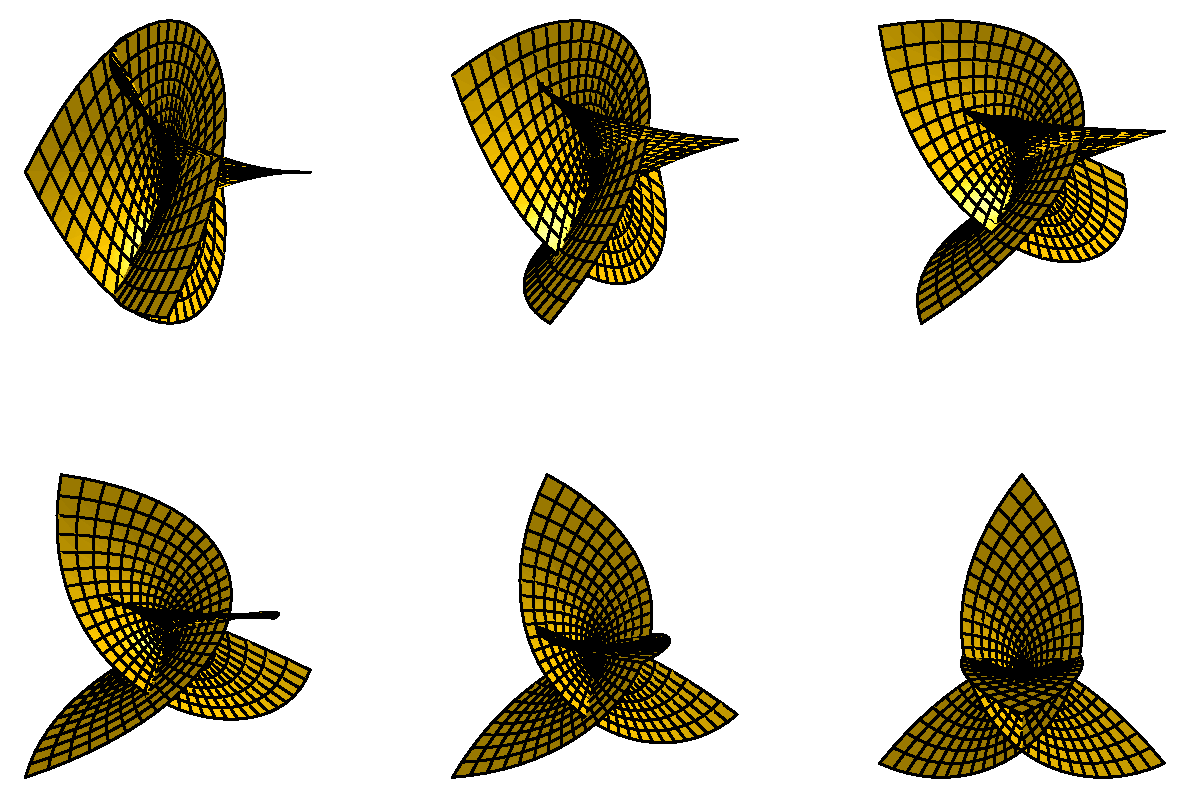
\includegraphics[width=12cm]{Images/EnneperFamily.eps}
   \caption{The Enneper Family of Minimal Surfaces}
   \label{fig:enneper}
\end{figure}

\end{example} 

\subsection{The Weierstrass-Enneper Representation}
\label{WERep}
We know all surfaces can be isothermally parametized (\ref{defisothermal}) and if an isothermally parametrised surface is minimal then its coordinate functions are harmonic (\ref{harmonic}).

Let $\mathbf x(u,v)$ be a minimal surface with an isothermal parametrisation (Section \ref{isothermal})

Then let $\mathbf y$ be the harmonic conjugate of $\mathbf x$.

Using the complex variable $z = u + iv$ we can write
\begin{displaymath}
\mathbf f(z) = \mathbf x + i \mathbf y \mbox{\ \ is holomorphic}
\end{displaymath}

Now define $\mathbf \Phi$ as

\begin{displaymath}
\mathbf \Phi = \frac{\partial \mathbf f}{\partial z} = \frac{1}{2}(\mathbf x_u + i \mathbf y_u) \stackrel{\ref{CR}}{=} \frac{1}{2}(\mathbf x_u - i \mathbf x_v) 
\label{Phi}
\end{displaymath}

\begin{theorem}
If $\mathbf \Phi: U \rightarrow \mathbb R^3$ is an isothermally parametrised minimal surface, the vector-valued holomorphic function $\mathbf \Phi=(\Phi_1, \Phi_2, \Phi_3)$ defined above satisfies the following conditions:
\begin{enumerate}
	\item $\Phi_1^2+\Phi_2^2+\Phi_3^2 = 0$ 
	\item $\mathbf \Phi$ is nowhere zero.
\end{enumerate}
\end{theorem}

\begin{proof}
\begin{eqnarray}
\nonumber
\sum_{k=1}^3 \Phi_k^2 &=& \sum_{k=1}^3 \frac{1}{4}\left(x_u^k - i x_v^k \right) \\
\nonumber
&=& \frac{1}{4}(\mathbf x_u \cdot \mathbf x_u - \mathbf x_v \cdot \mathbf x_v - 2i \mathbf x_u \cdot \mathbf x_v) \\
\nonumber
&=& \frac{1}{4}(E - G - 2i F) \\
\nonumber
&=& 0 \mbox{\ \ by definition of isothermal paramatization (\ref{defisothermal})}
\end{eqnarray}
Finally $\mathbf \Phi = \vec 0$ iff $\mathbf x_u = \mathbf x_v = 0$ which is impossible since $\mathbf x$ is regular.
\end{proof}

Now if we define

\begin{displaymath}
g(z) = \frac{\Phi_3}{\Phi_1-i\Phi_2} \mbox{\ and \ } f(z) = \Phi_1-i\Phi_2
\end{displaymath} 

Manipulating these gives:

\begin{eqnarray}
\nonumber
\Phi_1 &=& \frac{1}{2}(1-g^2)f \\
\nonumber
\Phi_2 &=& \frac{i}{2}(1+g^2)f \\
\nonumber
\Phi_3 &=& fg\\
\end{eqnarray}

Note these satisfy $\Phi_1^2+\Phi_2^2+\Phi_3^2 = 0$.
 
We can take a path independent contour integral for each $\Phi_i$ with respect to z. The real part of which will be our isothermally parametrised minimal surface $\mathbf x(u,v)$ and the imaginary part will be the harmonic conjugate minimal surface, $\mathbf y(u,v)$.\\
Conditions on g:
\begin{enumerate}
	\item Meromorphic
\end{enumerate}
Conditions on f:
\begin{enumerate}
	\item Holomorphic
	\item If g has a pole of order $m \geq 1$ at $z_0$ then f has a zero of order $n \geq 2m$ at $z_0$.
\end{enumerate}

\begin{example}
To demonstrate the ease with which we can now produce minimal surfaces we will take,
\begin{displaymath}
f(z) = z \ \ \ \ g(z) = z
\end{displaymath}

So 

\begin{eqnarray}
\nonumber
\Phi_1 &=& \frac{1}{2}(1-z^2)z \\
\nonumber
\Phi_2 &=& \frac{i}{2}(1+z^2)z \\
\nonumber
\Phi_3 &=& z^2
\end{eqnarray}

Then
\begin{eqnarray}
\nonumber
x^1(z,\bar{z}) &=& \Re \int \Phi_1 dz \\
\nonumber
&=& \Re \left(\frac{1}{8}(2z^2-z^4)\right) \mbox{\ \ \ \ Now sub in for } z=u+iv \\
\nonumber
&=& -\frac{1}{4}u^4+\frac{3}{2}u^2v^2-\frac{1}{4}v^4+\frac{1}{2}u^2-\frac{1}{2}v^2
\end{eqnarray}

\begin{eqnarray}								
\nonumber
x^2(z,\bar{z}) &=& \Re \int \Phi_2 dz \\
\nonumber
&=& \Re \left(\frac{i}{8}(2z^2+z^4)\right) \mbox{\ \ \ \ Now sub in for } z=u+iv \\
\nonumber
&=& u^3v+uv^3-uv
\end{eqnarray}

\begin{eqnarray}								
\nonumber
x^3(z,\bar{z}) &=& \Re \int \Phi_3 dz \\
\nonumber
&=& \Re \left(\frac{z^3}{3}\right) \mbox{\ \ \ \ Now sub in for } z=u+iv \\
\nonumber
&=& \frac{2}{3}u^3-2v^2u
\end{eqnarray} 
\end{example}

So we have a minimal surface $\mathbf x(u,v) = (x^1,x^2,x^3)$ which is shown in Figure \ref{fig:WEExample}.

\begin{figure}[htbp]
	\centering
       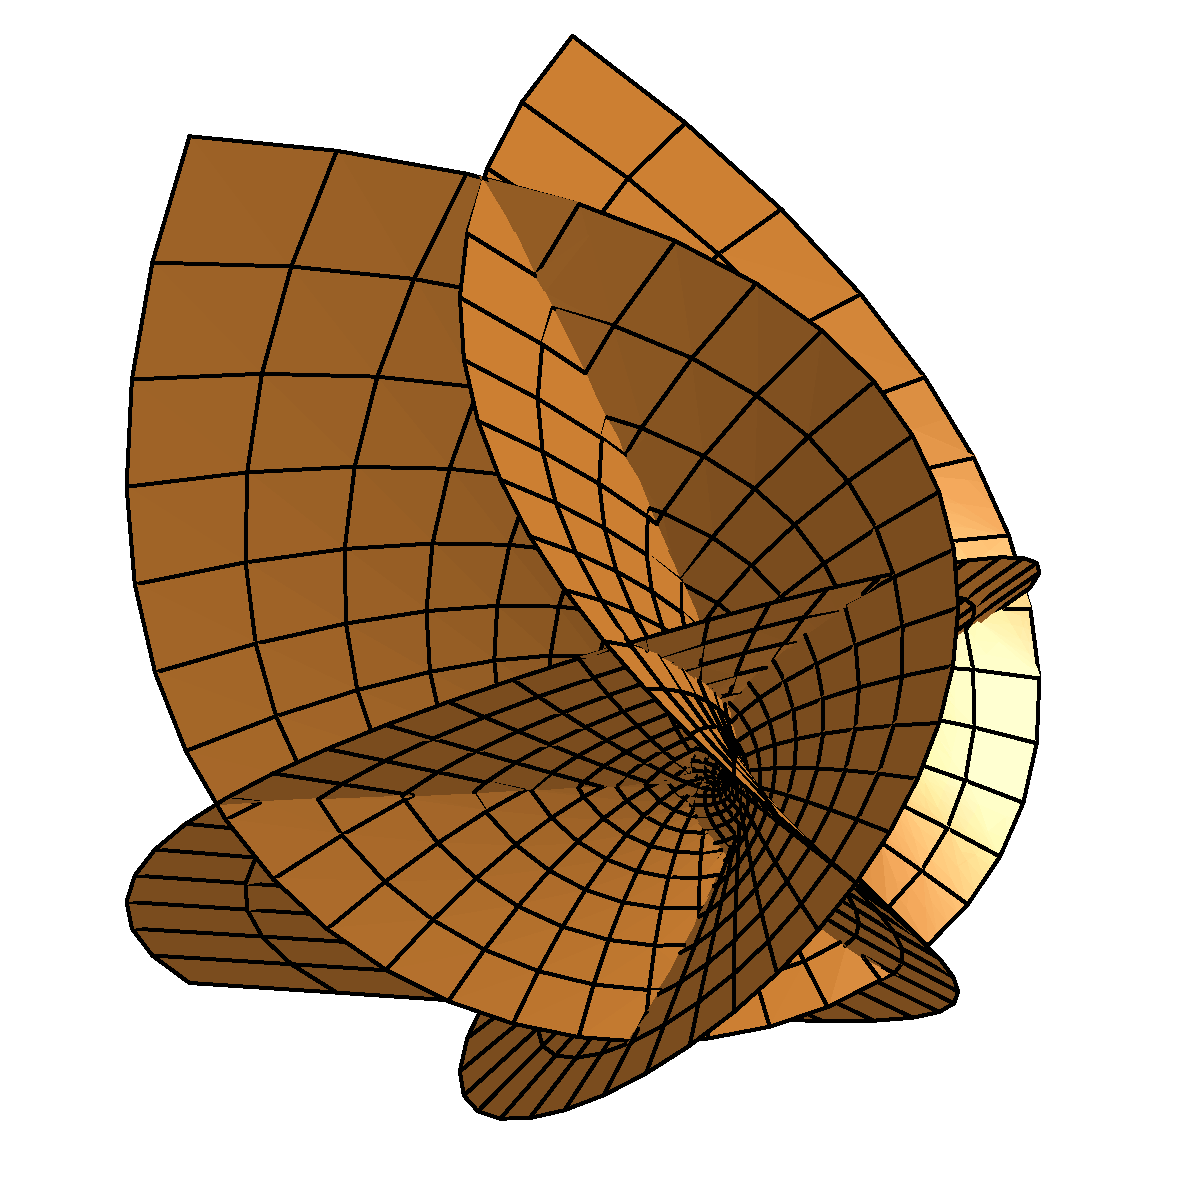
\includegraphics[width=8cm]{Images/WEExample.eps}
   \caption{Minimal Surface Generated by $f(z) = z$ and $g(z) = z$}
   \label{fig:WEExample}
\end{figure}


 


\newpage
\section{The Gauss Map}
The Gauss map is deeply embedded in Minimal Surface Theory. This section requires knowledge of the preceding sections on Complex Analysis, Isothermal Parametrisation and the Weierstrass-Enneper Representation.

\subsection{Conformal Maps}
These are maps which preserve angle. A Linear transformation $T:\mathbb R^2 \rightarrow \mathbb R^2$ is conformal if, for fixed $\rho > 0$
\begin{displaymath}
T(\mathbf x) \cdot T(\mathbf y) = \rho^2 \mathbf x \cdot \mathbf y
\end{displaymath}

In relation to surfaces this implies that if a map between surfaces is conformal then the angles between tangent vectors are preserved through the map.

This can be seen from $\mathbf x \cdot \mathbf y = |\mathbf x||\mathbf y|\cos \theta$

\subsection{Tangent Vectors through the Gauss Map}
The Gauss map of a surface $M$ with parametrisation $\mathbf x(u,v)$ is a mapping from the surface to the unit sphere, denoted $G:M \rightarrow S^2$ and given by $G(p)=\mathbf N_p$ where $\mathbf N_p$ is the unit normal to M at p.

Now in order to see how angles are affected by the Gauss map we need to be able to transform tangent spaces through the Gauss map. The Gauss map as defined, takes a point p on the surface to a point q on $S^2$ via the unit normal to the surface. So if at point p we have a tangent plane, the unit normal is perpendicular to this; however due to the properties of the sphere the tangent plane at q on the sphere is also perpendicular to the same unit normal therefore the Gauss map, maps tangent planes onto themselves.

We can therefore write $G_*(\mathbf x_u)=N_u$ and $G_*(\mathbf x_v) = \mathbf N_v$



\subsection{Minimal iff Gauss Map Anti-Conformal}
\begin{theorem}
The Gauss Map of a surface M is Anti Conformal if and only if M is Minimal.
\label{GMAntiC}
\end{theorem}

\subsubsection{What does this mean?}
If we have a surface then we can find curves on the surface that intersect. If we use the Gauss map to take each point on the curves to a point on $S^2$ we get new curves on $S^2$.

By taking the tangent vectors at the points of intersection we can find the angle between the curves. If the angle between our original curves and our mapped curves is the same then the Gauss Map is said to be conformal for our surface.

Anti conformal simply means that while the angle between the curves is the same they've swapped orientation (eg instead of rotating curve 1 clockwise to get to curve 2, you now rotate curve 2 clockwise to get to curve 1.)

\subsubsection{Formulae required for the proof.}
Throughout we shall work in Isothermal Coordinates:
\begin{displaymath}
E=G \mbox{\ \ \ \ } F=0
\end{displaymath}
Also we need the basis expansion for the derivatives of the Gauss Map:

\begin{eqnarray}
\nonumber
G_*(\mathbf x_u) = \mathbf N_u &=& -\frac{L}{E} \mathbf x_u - \frac{M}{G} \mathbf x_v \\
G_*(\mathbf x_v) = \mathbf N_v &=& -\frac{M}{E} \mathbf x_u - \frac{N}{G} \mathbf x_v
\label{GMBE}
\end{eqnarray}

Lastly we need the formula for the Mean curvature of a surface parametrised by isothermal coordinates:

\begin{displaymath}
H = \frac{L+N}{2E} \mbox{\ \ \ } \left(\mbox {Eg \ } H=0 \Leftrightarrow L=-N \right)
\end{displaymath}

\subsubsection{Formal Proof}

\begin{prop}
Surface M, Minimal $\Rightarrow$ Gauss Map of M conformal.
\end{prop}

\begin{proof}

Need to show:
\begin{enumerate}
\item \begin{displaymath}
G_*(\mathbf x_u) \cdot G_*(\mathbf x_v) = \rho^2(u,v)\mathbf x_u \cdot \mathbf x_v
\end{displaymath}
\begin{eqnarray}
\nonumber
LHS &=& G_*(\mathbf x_u) \cdot G_*(\mathbf x_v) \\
\nonumber
&=& \mathbf N_u \cdot \mathbf N_v \\
\nonumber
&=& \left(-\frac{L}{E} \mathbf x_u - \frac{M}{E} \mathbf x_v \right) \cdot \left(-\frac{M}{E} \mathbf x_u - \frac{N}{E} \mathbf x_v \right) \\
\nonumber
&=& M\left(L+N\right) = 0 \mbox{\ \ \ \ \ since M minimal} \\
\nonumber
&=& \rho^2(u,v) G \mbox{\ \ \ \ \ Since G=0} \\
\nonumber
&=& \rho^2(u,v)\mathbf x_u \cdot \mathbf x_v = RHS
\end{eqnarray}   

\item \begin{displaymath}
G_*(\mathbf x_u) \cdot G_*(\mathbf x_u) = \rho^2(u,v)\mathbf x_u \cdot \mathbf x_u
\end{displaymath}
\begin{eqnarray}
\nonumber
G_*(\mathbf x_u) \cdot G_*(\mathbf x_u)&=& \mathbf N_u \cdot \mathbf N_u \\
\nonumber
&=& \left(-\frac{L}{E} \mathbf x_u - \frac{M}{E} \mathbf x_v \right) \cdot \left(-\frac{L}{E} \mathbf x_u - \frac{M}{E} \mathbf x_v \right) \\
\nonumber
&=& \frac{L^2}{E} + \frac{M^2}{E} = \rho^2 E
\end{eqnarray} 
\begin{displaymath}
\Leftrightarrow \rho^2 = \frac{L^2+M^2}{E^2}
\end{displaymath}

\item \begin{displaymath}
G_*(\mathbf x_v) \cdot G_*(\mathbf x_v) = \rho^2(u,v)\mathbf x_v \cdot \mathbf x_v
\end{displaymath}
\begin{eqnarray}
\nonumber
G_*(\mathbf x_v) \cdot G_*(\mathbf x_v) &=& \mathbf N_v \cdot \mathbf N_v \\
\nonumber
&=& \left(-\frac{M}{E} \mathbf x_u - \frac{N}{E} \mathbf x_v \right) \cdot \left(-\frac{M}{E} \mathbf x_u - \frac{N}{E} \mathbf x_v \right) \\
\nonumber
&=& \frac{M^2}{E} + \frac{N^2}{E} = \rho^2 E
\end{eqnarray} 
\begin{displaymath}
\Leftrightarrow \rho^2 = \frac{N^2+M^2}{E^2}
\end{displaymath}

\end{enumerate}

Since M is minimal we know $L = -N$, therefore $\rho^2$ is equal in (1), (2) and (3).
\end{proof}

\begin{prop}
Surface M has anti-conformal Gauss Map $\Rightarrow$ M Minimal.
\end{prop}

\begin{proof}
Gauss map is conformal so we know from the definition
\begin{displaymath}
G_*(\mathbf x_u) \cdot G_*(\mathbf x_v) = \rho^2(u,v)\mathbf x_u \cdot \mathbf x_v
\end{displaymath}

Remember we are working in isothermal coordinates so we have 
\begin{displaymath}F = \mathbf x_u \cdot \mathbf x_v = 0\end{displaymath}

\begin{displaymath}
\mathbf N_u \cdot \mathbf N_v = M(L+N) = 0
\end{displaymath}

So either L=-N in which case the surface is minimal and we are done or if this is not the case then we must have $M=0$.

Subbing $M=0$ into equations for $\mathbf N_u \cdot \mathbf N_u$ and $\mathbf N_v \cdot \mathbf N_v$ we know

\begin{eqnarray}
\nonumber
\mathbf N_u \cdot \mathbf N_u &=& \frac{L^2}{E} = \rho^2 E \\
\nonumber
\mathbf N_v \cdot \mathbf N_v &=& \frac{N^2}{E} = \rho^2 E
\end{eqnarray}

So

\begin{displaymath}
\frac{L^2}{E^2} = \rho^2 = \frac{N^2}{G^2} \Rightarrow \frac{L}{E} = \pm \frac{N}{G} 
\end{displaymath}

Setting $\frac{L}{E} = \frac{N}{G} = \kappa$ we can use the basis expansion (\ref{GMBE}) to write down the matrix for the differential of the Gauss Map for the two possibilities (e.g. the $\pm$).

\begin{displaymath}
\mathbf{dN_p} =
\left( \begin{array}{cc}
\kappa & 0 \\
0 & \pm \kappa
\end{array} \right)
\end{displaymath}

The principal curvatures are given by the determinant of $\mathbf{dN_p}$ so we have two cases:
\begin{enumerate} 
\item Principal curvatures $(\kappa, \kappa) \Rightarrow$ a Sphere (Note not anti conformal as this matrix does not reverse orientation).
\item Principal curvatures $(\kappa, -\kappa) \Rightarrow$ minimal surface ($H = \frac{\kappa_1 + \kappa_2}{2} = \frac{\kappa - \kappa}{2} = 0$) (Note anti conformal since this matrix reverses orientation!)
\end{enumerate}
\end{proof}

Putting these two directions together proves \ref{GMAntiC}.


\subsection{The Gauss Map in terms of the Weierstrass \\ Representation}

The Gauss Map is further linked to minimal surfaces through the Weierstrass-Enneper representation.
\begin{theorem}
Let M be a conformally parametrised surface with Weierstrass-Enneper representation (f,g). Then the Gauss map of M, $G: M \rightarrow \mathbb C \cup \left\{ \infty \right\}$, may be identified with the meromorphic function g.
\end{theorem}

In order to provide a proof we first need to introduce a parametrisation of the sphere (since the Gauss map maps our surface onto the sphere) known as Stereographic Projection.

\begin{definition}[Stereographic Projection]
Stereographic projection maps each point of the sphere onto the plane by projection from the North pole (N). This map is denoted by:

\begin{displaymath}
St: S^2/{N} \rightarrow \mathbb R^2
\end{displaymath}

and for the standard parametrisation of a sphere is defined by 

\begin{displaymath}
St(\cos u \cos v, \sin u \cos v, \sin v) = \left(\frac{\cos u \cos v}{1-\sin v}, \frac{\sin u \cos v}{1-\sin v}, 0 \right)
\end{displaymath}
\end{definition}

This becomes clear if we look at figure \ref{fig:stereographic}.

Furthermore as with the Gauss Map we can take the induced mapping on tangent vectors by differentiating with respect to u and v giving:

\begin{eqnarray}
\nonumber
St_*(\mathbf x_u) &=& \left(\frac{-\sin u \cos v}{1-\sin v},\frac{\cos u \cos v}{1-\sin v}, 0 \right) \\
\nonumber
St_*(\mathbf x_v) &=& \left(\frac{\cos u}{1-\sin v},\frac{\sin u}{1-\sin v}, 0 \right)
\end{eqnarray}

\begin{figure}[htbp]
	\centering
       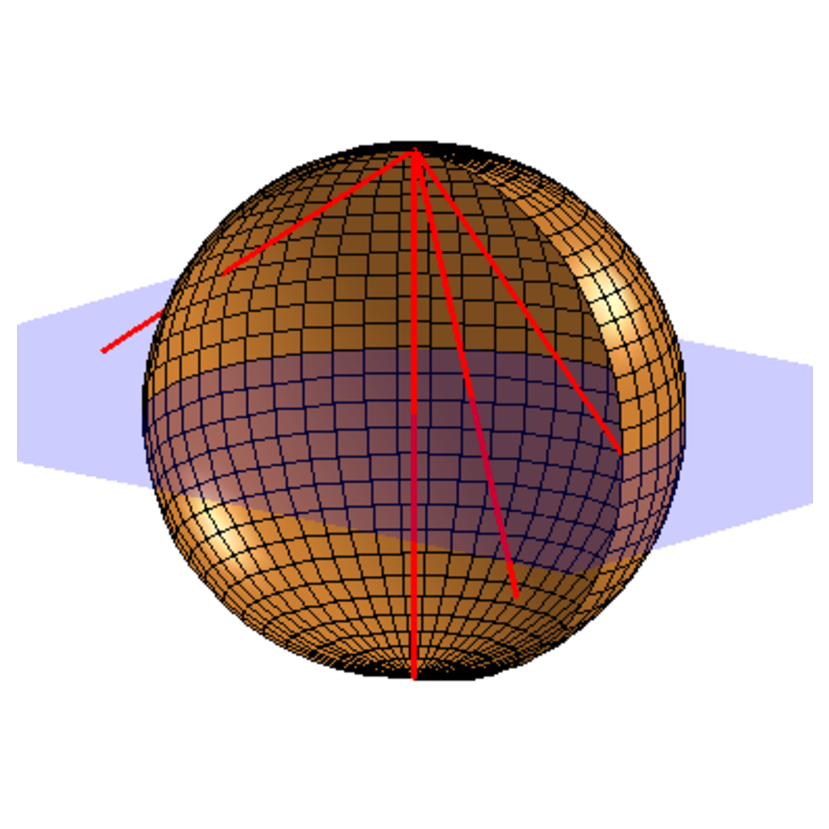
\includegraphics[width=8cm]{Images/Stereographic.eps}
   \caption{Stereographic Projection}
   \label{fig:stereographic}
\end{figure} 

\begin{proof}{(\cite{OPR} Page 92)}
From section \ref{WERep} recall that $\Phi = \frac{\partial \mathbf x}{\partial z}$, $\bar{\Phi} = \frac{\partial \mathbf x}{\partial \bar{z}}$ and

\begin{eqnarray}
\nonumber
\Phi^1 &=& \frac{1}{2}(1-g^2)f \\
\nonumber
\Phi^2 &=& \frac{i}{2}(1+g^2)f \\
\nonumber
\Phi^3 &=& fg\\
\end{eqnarray}

Our aim is to describe the Gauss map in terms of $\Phi^1$, $\Phi^2$ and $\Phi^3$

So take

\begin{eqnarray}
\nonumber
\mathbf x_u \times \mathbf x_v &=& ((\mathbf x_u \times \mathbf x_v)^1,(\mathbf x_u \times \mathbf x_v)^2,(\mathbf x_u \times \mathbf x_v)^3) \\
\nonumber
&=& (x_u^2x_v^3 - x_u^3x_v^2, x_u^3x_v^1-x^1_ux^3_v,x^1_ux^2_v-x^2_ux^1_v)
\end{eqnarray}

Taking the first component $(\mathbf x_u \times \mathbf x_v)^1 = x_u^2x_v^3 - x_u^3x_v^2$, (Recalling \ref{Phi}) we now write it in terms of components of $\Phi$.

\begin{eqnarray}
\nonumber
x_u^2x_v^3 - x_u^3x_v^2 &=& \Im[(x_u^2-ix_v^2)(x_u^3+ix_v^3)] \\
\nonumber 
&=& \Im\left[2\left(\frac{\partial x^2}{\partial z}\right)\cdot 2\left(\frac{\partial x^3}{\partial\bar{z}}\right)\right] \\
\nonumber
&=& 4 \Im(\Phi^2\bar{\Phi}^3)
\end{eqnarray} 
Following the same process we get
\begin{eqnarray}
\nonumber
(\mathbf x_u \times \mathbf x_v)^2 &=& 4 \Im(\Phi^3\bar{\Phi}^1) \\ 
\nonumber
(\mathbf x_u \times \mathbf x_v)^3 &=& 4 \Im(\Phi^1\bar{\Phi}^2)
\end{eqnarray}

And so we obtain
\begin{displaymath}
\mathbf x_u \times \mathbf x_v = 4 \Im(\Phi^2\bar{\Phi}^3,\Phi^3\bar{\Phi}^1,\Phi^1\bar{\Phi}^2) = 2(\Phi \times \bar{\Phi})
\end{displaymath}
since $z-\bar{z} = 2 \Im z$.

Now given that $\mathbf x(u,v)$ is isothermal

\begin{displaymath}
|\mathbf x_u \times \mathbf x_v| = |\mathbf x_u| \cdot |\mathbf x_v| = |\mathbf x_u|^2 = E = 2|\Phi|^2.
\end{displaymath}

Therefore

\begin{displaymath}
\mathbf N = \frac{\mathbf x_u \times \mathbf x_v}{|\mathbf x_u \times \mathbf x_v|} = \frac{2(\Phi \times \bar{\Phi})}{2|\Phi|^2} = \frac{\Phi \times \bar{\Phi}}{|\Phi|^2}
\end{displaymath}

We are now half way there, having written the unit normal in terms of $\Phi$.

Now using Stereographic projection we write the Gauss map $G:M\rightarrow \mathbb C \cup \infty$ in terms of the $\Phi^i$:

\begin{eqnarray}
\nonumber
G(\mathbf x(u,v)) &=& \mbox{St }(\mathbf N(u,v)) \\
\nonumber
&=& \mbox{St }\left(\frac{\Phi \times \bar{\Phi}}{|\Phi|^2}\right) \\
\nonumber
&=& \mbox{St }\left(\frac{2\Im(\Phi^2\bar{\Phi}^3,\Phi^3\bar{\Phi}^1,\Phi^1\bar{\Phi}^2)}{|\Phi|^2}\right) \\
\nonumber
&=& \left(\frac{2\Im(\Phi^2\bar{\Phi^3})}{|\Phi|^2-2\Im(\Phi^1\bar{\Phi}^2)}, \frac{2\Im(\Phi^3\bar{\Phi^1})}{|\Phi|^2-2\Im(\Phi^1\bar{\Phi}^2)}, 0 \right)
\end{eqnarray}

The last equality follows because

\begin{eqnarray}
\nonumber
\frac{x}{1-z} &=& \frac{2\Im(\Phi^2\bar{\Phi}^3)}{|\phi|^2}\cdot\frac{1}{1-\frac{2\Im(\Phi^2\bar{\Phi}^3)}{|\phi|^2}} \\
\nonumber
&=&\frac{2\Im(\Phi^2\bar{\Phi}^3)}{|\phi|^2}\cdot \frac{|\Phi|^2}{|\Phi|^2-2\Im(\Phi^1\bar{\Phi^2})} \\
\nonumber
&=& \frac{2\Im(\Phi^2\bar{\Phi^3})}{|\Phi|^2-2\Im(\Phi^1\bar\Phi^2)}
\end{eqnarray}
similarly for $\frac{y}{1-z}$. Identifying $(x,y) \in \mathbb R^2$ with $x+iy \in \mathbb C$ allows us to write
\begin{displaymath}
G(\mathbf x(u,v)) = \frac{2\Im(\Phi^2\bar{\Phi}^3)+2i\Im(\Phi^3\bar{Phi}^1)}{|\Phi|^2-2\Im(\Phi^1\bar{\Phi}^2)}
\end{displaymath}

Now, considering the numerator $N$ of this fraction:

\begin{eqnarray}
\nonumber
N &=& 2\Im(\Phi^2\bar{Phi}^3) + 2i\Im(\Phi^3\bar{Phi}^1) \\
\nonumber
&=& \frac{1}{i}[\Phi^2\bar{Phi}^3-\bar{\Phi}^2\Phi^3+i\Phi^3\bar{Phi}^1-i\bar{\Phi}^3\Phi^1] \\
\nonumber
&=& \Phi^3(\bar{\Phi}^1+i\bar{\Phi}^2)-\bar{\Phi}^3(\Phi^1+i\Phi^2)
\end{eqnarray}

Also
\begin{displaymath}
0 = (\Phi)^2 =(\Phi^1)^2+(\Phi^2)^2+(\Phi^3)^2 = (\Phi^1-i\Phi^2)(\Phi^1+i\Phi^2)+(\Phi^3)^2
\end{displaymath}
so
\begin{displaymath}
\Phi^1 + i \Phi^2 =\frac{-(\Phi^3)^2}{\Phi^1-i\Phi^2}
\end{displaymath}

Then we have
\begin{eqnarray}
\nonumber
N &=& \Phi^3(\bar{\Phi}^1+i\bar{\Phi}^2)+\bar{\Phi}^3\frac{(\Phi^3)^2}{\Phi^1-i\Phi^2} \\
\nonumber
&=&\frac{\Phi^3[(\Phi^1-i\Phi^2)(\bar{\Phi}^1+i\bar{\Phi}^2)+|\Phi^3|^2]}{\Phi^1-i\Phi^2} \\
\nonumber
&=& \frac{\Phi^3}{\Phi^1-i\Phi^2}[|\Phi^1|^2+|\Phi^2|^2+|\Phi^3|^2 + i(\bar{\Phi}^2\phi^1-\Phi^2\bar{\Phi}^1)] \\
\nonumber
&=& \frac{\Phi^3}{\Phi^1-i\Phi^2} [|\Phi|^2 - 2\Im(\Phi^1\bar{\Phi}^2)]
\end{eqnarray}

The second factor of the numerator $N$ cancels the denominator of $G(\mathbf x(u,v))$, and we end up with

\begin{displaymath}
G(\mathbf x(u,v))=\frac{\Phi^3}{\Phi^1-i\Phi^2}
\end{displaymath}

Which is our definition for $g(z)$ (given in Section \ref{WERep}) as required.
\end{proof}
\newpage
\section{A Generalisation of the Helicoid}

In this section I will review \cite{BLR} a paper entitled \emph{A Generalization of the Helicoid} written by D. E. Blair and J. R. Vanstone in 1978.

We will begin by stating the theorem and then explaining what it means before giving an expanded version of the proof with more explanation than is given in \cite{BLR}.

\begin{nonumbertheorem}
Let $M^n$ be a complete minimal hypersurface of $E^{n+1}$ and suppose that $M^n$ admits a codimension 1 foliation by Euclidean $(n-1)$ spaces. Then either $M^n$ is totally geodesic or $M^n =  M^2 \times E^{n-2}$ where $M^2$ is a Helicoid in $E^3$.
\cite{BLR}
\end{nonumbertheorem}

Clearly a good place to start is with some definitions!

\subsection{Definitions}

\begin{definition}[Complete]
A surface which has no edges.
\end{definition}

\begin{definition}[Hypersurface]
A hypersurface is a generalization of a 2 dimensional surface to an n-dimensional surface embedded in (n+1)-dimensional space.

They are the set of the solutions to the equation:

\begin{displaymath}
f(x_1 + x_2 + ... + x_n) = 0 \mbox{\ \ \ \ embedded in } E^{n+1}
\end{displaymath}

\end{definition}

\begin{definition}[Codimension]
The codimension is the difference between the dimension of one (geometric or algebraic) object and the dimension of a smaller object contained in it.
\end{definition}

\begin{definition}[Foliation]
The idea of a foliation is easiest to grasp in $E^2$ and $E^3$ dimension to begin with.
For instance if we take $E^2$ minus the origin then a series of concentric circles foliate this space.
Likewise in $E^3$ minus the origin taking a series on concentric spheres foliates this space.
So the theorem requires that there exists a foliation of $M^n$ by objects of dimension $(n-1)$
\end{definition}

\begin{definition}[Totally Geodesic]
A hypersurface is totally geodesic if all of its geodesics are also geodesics of the ambient space.
\end{definition}

The theorem is therefore saying that if we have a hypersurface $M^n$ that we can foliate with objects of dimension $(n-1)$ then either $M^n$ is totally geodesic or $M^n = M^2 \times R^{n-2}$ where $M^2$ is a Helicoid in $E^3$

The exciting thing about this theorem is that it is in fact an extension of theorem \ref{Ruled} which says that in $E^3$ the only ruled surface apart from the plane is a Helicoid. A ruled surface (dimension n=2) is one that can be foliated by straight lines (dimension n=1) therefore a ruled surface admits a codimension 1 foliation. According to our theorem then such a minimal surface must either be totally geodesic which in $mathbb R^3$ means it has to be the plane or $M^2 \times E^0 = M^2$ which is the Helicoid.


\subsection{Necessary Tools for the Proof}
Before we begin to get to grips with the proof we need to review and introduce some notation and some tools.

\begin{enumerate}
	\item The Lie bracket $[X,Y] = \mathbf D_X Y - \mathbf D_Y X$
	\item If $(x^1,...,x^n)$ is a coordinate system then $\left[ \frac{\partial}{\partial x^i},\frac{\partial}{\partial x^j} \right] = 0$ - commuting partial derivatives.
	\item If $X,Y$ are uniform and tangential to a foliation then $[X,Y]$ is also tangential to the foliation
\end{enumerate}

We also need some rules for manipulating covariant derivatives.

$\mathbf D_x Y$ is linear in $X$ so
\begin{itemize}
	\item $\mathbf D_{X+Z}Y = \mathbf D_x Y + \mathbf D_z Y$
	\item $\mathbf D_{\alpha X}Y = \alpha \mathbf D_x Y$
	\item $\mathbf D_x(Y_1+Y_2)=\mathbf D_x Y_1 + \mathbf D_x Y_2$
	\item $\mathbf D_{\frac{\partial}{\partial X^i}} (\alpha Y) = \frac{\partial \alpha}{\partial X^i} Y + \alpha \mathbf D_{\frac{\partial}{\partial X^i}} Y$
\end{itemize}

\subsection{The Proof}
Firstly we need to set up some notation.

Let D be the Riemannian connection on $E^{n+1}$ and by $g$ and $\nabla$ the induced Riemannian metric and connection on $M^n$.

We'll use local coordinates $(t,x^1,...,x^n)$ such that

\begin{displaymath}
X_i = \frac{\partial}{\partial x^i} \mbox{\, \, \, \,} U = \alpha \frac{\partial}{\partial t}
\end{displaymath}
for some function $\alpha$
where $U$ is a unit vector field which together with $X_i$ forms and orthonormal basis such that $\mathbf D_{X_i}X_j = 0$

At this point we need to note an important difference between the notation we will use and the notation that the papers authors use. In their original paper they have coordinates $(t,x^2,...,x^n)$ and then every time they sum over the $x_i$'s they use $\sum_{i=2}^n$. Instead we will use standard \emph{Einstein Summation Notation} e.g. summing over repeated indices. Therefore indices will run from 1 to n unless otherwise specified (note that for convenience, in places $X_0 = \frac{\partial \ }{\partial t}$).

Then calculating the Lie bracket for this distribution 
\begin{eqnarray}
\nonumber
[U, Xi] &=& \mathbf D_U X_i - \mathbf D_{X_i} U \\
\nonumber
&=& \mathbf D_{\alpha \frac{\partial}{\partial t}} \frac{\partial}{\partial x^i} - \mathbf D_{\frac{\partial}{\partial x^i}}  \alpha \frac{\partial}{\partial t} \\
\nonumber
&=& \alpha \mathbf D_{\frac{\partial}{\partial t}}\frac{\partial}{\partial x^i}- \frac{\partial \alpha}{\partial x^i}\frac{\partial}{\partial t} - \alpha \mathbf D_{\frac{\partial}{\partial x^i}}\frac{\partial}{\partial t} \\
\nonumber
&=& \alpha \left[\frac{\partial}{\partial t},\frac{\partial}{\partial x^i}\right] - \frac{\partial \alpha}{\partial x^i}\frac{\partial}{\partial t} \\
\nonumber
&=& - \frac{\partial \alpha}{\partial x^i}\frac{\partial}{\partial t} \\
\nonumber
&=& - \frac{\partial \ln \alpha}{\partial x^i}\alpha\frac{\partial}{\partial t} \mbox{\ \ \ \ Letting } p = \ln \alpha \\
\nonumber
&=& -(X_i p)X
\end{eqnarray}

\begin{equation}
\framebox{$[U,X_i] = -(X_i p)U$ \ \ \ \ where $p = \ln \alpha$} 
\label{IntUXi}
\end{equation}

Since $(X_ip)U$ is tangential to the distribution, this means that the distribution is integrable. Basically this allows us to say that the distribution is \emph{smooth} and so the distribution is in fact a foliation.

Given the above coordinates and vector fields we can construct a metric:
\begin{eqnarray}
\nonumber
g_{00}&=&\frac{\partial}{\partial t} \cdot \frac{\partial}{\partial t} = \frac{1}{\alpha^2}|U|= \frac{1}{\alpha^2} \mbox{ since U is a unit vector field.} \\
\nonumber
\mbox{For $\mu \neq \nu$ } g_{\mu \nu}&=&\frac{\partial}{\partial x^\mu} \cdot \frac{\partial}{\partial x^\nu} = 0 \mbox{ since orthonormal.} \\
\nonumber
\mbox{For $\mu=\nu > 1$ } g_{\mu \nu}&=&\frac{\partial}{\partial x^\mu} \cdot \frac{\partial}{\partial x^\nu} = 1 \mbox{ since $X_j$ are unit vector fields.}
\end{eqnarray}
Giving
\begin{displaymath}
g_{\mu \nu} = 
\left(\begin{array}{clrrrr}      
\frac{1}{\alpha^2} &   &  &  &  & 0\\       
  								 & 1 &   & & &  \\ 
  								 &   & . &  & &  \\ 
  								 &   &   & . &  &  \\ 
  								 &   &   &   & . &  \\ 
  		0						 &  &  & & & 1  
\end{array}\right)
\mbox{\, \, \, \,} g^{\mu \nu} = 
\left(\begin{array}{clrrrr}      
\alpha^2 &   &  &  &  & 0\\       
  								 & 1 &   & & &  \\ 
  								 &   & . &  & &  \\ 
  								 &   &   & . &  &  \\ 
  								 &   &   &   & . &  \\ 
  		0						 &  &  & & & 1  
\end{array}\right)
\end{displaymath}

We now wish to calculate the $\nabla$ connections which are covariant derivatives on $M^n$.

To do this we use \emph{Theorem Egregium} to express everything in terms of the first fundamental form.

In particular we'll use the following:

\begin{equation}
\framebox{$\nabla_{X_i}X_j = \Gamma^k_{ij}X_k = \Gamma_{ijl}g^{lk}X_k = \frac{1}{2}(g_{il,j}+g_{jl,i}-g_{ij,l})g^{lk}X_k$}
\end{equation}

\begin{eqnarray}
\nonumber
\nabla_{X_i}X_j &=& \nabla_{\frac{\partial}{\partial x^i}}\frac{\partial}{\partial x^j} \\
\nonumber 
&=& \Gamma_{ij}^kX_k \\
\nonumber
&=& \Gamma_{ijl}g^{lk}X_k \\
\nonumber
&=& \frac{1}{2}(g_{il,j}+g_{jl,i}-g_{ij,l})g^{lk}X_k \mbox{\, \, \, $g^{\mu\nu}=0$ for $\mu \neq \nu$}\\
\nonumber
&=& \frac{1}{2}(g_{ik,j}+g_{jk,i}-g_{ij,k})g^{kk}X_k \\
\nonumber
&=& \frac{1}{2}(1_j+1_i-1_k)g^{kk}X_k \\
\nonumber
&=& 0
\end{eqnarray}
\begin{equation}
\framebox{$\nabla_{X_i}X_j = 0$}
\label{nXX}
\end{equation}

\begin{eqnarray}
\nonumber
\nabla_{X_i}U &=& \frac{\partial \alpha }{\partial x^i}  \frac{\partial}{\partial t} + \alpha \nabla_{\frac{\partial}{\partial x^i}}{\frac{\partial}{\partial t}} \\
\nonumber
&=& \frac{\partial \alpha }{\partial x^i}  \frac{\partial}{\partial t} + \alpha \Gamma^k_{i0}X_k \\
\nonumber
&=& \frac{\partial \alpha }{\partial x^i}  \frac{\partial}{\partial t} + \alpha \Gamma^{i0l}g^{lk}X_k \\
\nonumber
&=& \frac{\partial \alpha }{\partial x^i}  \frac{\partial}{\partial t} + \frac{\alpha}{2}(g_{il,0}+g_{0l,i}-g_{i0,l})g^{lk}X_k \\
\nonumber
&=& \frac{\partial \alpha }{\partial x^i}  \frac{\partial}{\partial t} + \frac{\alpha}{2}(g_{00,i}g^{00})X_0 \\
\nonumber
&=& \frac{\partial \alpha }{\partial x^i} \frac{\partial}{\partial t} + \frac{1}{2}\frac{\partial \frac{1}{\alpha^2}} {\partial x^i}\alpha^3\frac{\partial}{\partial t} \\
\nonumber
&=& \frac{\partial \alpha }{\partial x^i} \frac{\partial}{\partial t} - \frac{\partial \alpha} {\partial x^i}\frac{\partial}{\partial t} \\
\nonumber
&=& 0
\end{eqnarray}
\begin{equation}
\framebox{$\nabla_{X_i}U = 0$}
\label{nXU}
\end{equation}

\begin{eqnarray}
\nonumber
\nabla_UX_i &=& \nabla_{\alpha \frac{\partial}{\partial t}} \frac{\partial}{\partial x^i} \\ 
\nonumber
&=& \alpha \nabla_{\frac{\partial}{\partial t}}\frac{\partial}{\partial x^i} \\
\nonumber
&=& \alpha \Gamma_{0j}^k X_k \\
\nonumber
&=& \alpha \Gamma_{ijl}g^{lk} X_k \\
\nonumber
&=& \alpha \frac{1}{2}\left(g_{0l,j}+g_{jl,0}-g_{0j,l}\right)g^{lk} X_k \\
\nonumber
&=& \alpha \frac{1}{2}g_{00,j}g^{0k} X_k \mbox{\ \ \ \ (All $g_{ik,j}=0$ except for $g_{00,k}$) }\\
\nonumber
&=& \frac{\alpha}{2}\left[\frac{\partial}{\partial x^j}(\frac{1}{\alpha^2}) \alpha^2 \frac{\partial}{\partial t} \right] \\
\nonumber
&=& \frac{\alpha^2}{2}\left[\frac{\partial}{\partial x^j}(\frac{1}{\alpha^2}) X \right] \\
\nonumber
&=& \frac{1}{\alpha}\left[\frac{\partial \alpha}{\partial x^j} X \right] \\
\nonumber
&=& -\frac{1}{\alpha}\left[\frac{\partial \ln \alpha}{\partial x^j} \alpha X \right] \\
\nonumber
&=& - p_i X
\end{eqnarray}

\begin{equation}
\framebox{$\nabla_{U}X_i = -p_i X$}
\label{nUX}
\end{equation}

\begin{eqnarray}
\nonumber
\nabla_{U} U &=& \nabla_{\alpha \frac{\partial \ }{\partial t}}{\frac{\partial}\partial t} \\
\nonumber
&=&\alpha\nabla_{\frac{\partial \ }{\partial t}}\alpha \frac{\partial \ }{\partial t} \\
&=& \alpha \left[ \frac{\partial \alpha}{\partial t} \frac{\partial \ }{\partial t} + \alpha \mbox{\framebox{$\nabla_{\frac{\partial \ }{\partial t}}{\frac{\partial \ }{\partial t}}$}} \right ] \label{ntt}
\end{eqnarray}

Expanding the boxed covariant derivative:

\begin{eqnarray}
\nonumber
\nabla_{\frac{\partial \ }{\partial t}}{\frac{\partial \ }{\partial t}} &=& \Gamma_{00}^k X_k \\
\nonumber
&=& \Gamma_{00l}g^{lk}X_k \\
\nonumber
&=& \frac{1}{2}(g_{00,l}+g_{0l,0}-g{00,l})g^{lk}X_k \\
\nonumber
&=& \frac{1}{2} \left[g_{00,0}g^{00}X_0 - g_{00,1}g^{11} X_1 \ldots - g_{00,n}g^{nn} X_n \right] \\
\nonumber
&=& \frac{1}{2}\frac{\partial \ }{\partial t}\left(\frac{1}{\alpha^2}\right)\alpha^2\frac{\partial \ }{\partial t} - \frac{1}{2}  \frac{\partial \ }{\partial x^i}\left(\frac{1}{\alpha^2}\right)X_i \\
\nonumber
&=& -\frac{1}{\alpha}\frac{\partial \alpha}{\partial t}\frac{\partial \ }{\partial t} + \frac{1}{\alpha^3}\frac{\partial \alpha}{\partial x^i} X_i \\
\nonumber
&=& -\frac{1}{\alpha}\frac{\partial \alpha}{\partial t}\frac{\partial \ }{\partial t} + \frac{1}{\alpha^2}\frac{\partial \ln \alpha}{\partial x^i} X_i \\
\nonumber
&=& -\frac{1}{\alpha}\frac{\partial \alpha}{\partial t}\frac{\partial \ }{\partial t} + \frac{1}{\alpha^2} p_i X_i \\
\end{eqnarray}

Subbing this back in to \ref{ntt} gives us:

\begin{eqnarray}
\nonumber
\nabla_{U} U &=& \alpha \left[ \frac{\partial \alpha}{\partial t} \frac{\partial \ }{\partial t} + \alpha \mbox{\framebox{$\nabla_{\frac{\partial \ }{\partial t}}{\frac{\partial \ }{\partial t}}$}} \right ]  \\
\nonumber
&=& p_i X_i
\end{eqnarray}

\begin{equation}
\framebox{$\nabla_{U}U = p_i X_i$}
\label{nUU}
\end{equation}

We now introduce the Weingarten map which we define as

\begin{definition}[The Weingarten Map]
\begin{displaymath}
A(Y) = D_{\mathbf Y}\mathbf N
\end{displaymath}
\end{definition}

Now we apply the Weingarten map to our coordinates and expand via a basis expansion giving

\begin{equation}
\framebox{$A(U) = rU + q_i X_i, \ \ \ \ A (X_i) = q_i U$}
\label{Weingarten}
\end{equation}

Where $r$ and $q_i$ are some constants. We will use inner products to show that the $q_i$'s in both equations are equal and that $A(X_i)$ has zero $X_i$ component as shown. We can do this since $M^n$ is foliated by Euclidean (n-1)-dimensional spaces.

\begin{eqnarray}
\nonumber
<A(X_i), X_j> &=& <D_{X_i} \mathbf N, X_j> \\
\nonumber
&=& -<\mathbf N, D_{X_i}X_j> = 0
\end{eqnarray}

To show the $q_i$'s are the same in both equations we show
\begin{displaymath}
<A(X_i), U> = <A(U),X_i>
\end{displaymath}

So

\begin{eqnarray}
\nonumber
<A(X_i), U> &=& <D_{X_i} \mathbf N, U> \\
\nonumber
&=& -<N, D_{X_i}U> \\
\nonumber 
&=& -<N, D_U X_i - [U,X_i]>\\
\nonumber
&=& -<N, D_U X_i + X_i p U>\\
\nonumber
&=& -<N, D_U X_i>\\
\nonumber
&=& -<D_U N, X_i>
\end{eqnarray}

\begin{definition}[The Codazzi Equation]
\begin{displaymath}
(\nabla_X A)Y - (\nabla_{Y} A)X = 0
\end{displaymath}
For vector fields X and Y.

Where 
\begin{itemize}
	\item $(\nabla_X A) Y = \nabla_X(AY) - A(\nabla_X Y)$
	\item $(\nabla_Y A) X = \nabla_Y(AX) - A(\nabla_Y X)$
\end{itemize}
\end{definition}

So in our basis $(\nabla_U A) X_i - (\nabla_{X_i} A) U = 0$.

Plugging in from the definition and results shown previously:

\begin{align}
\nonumber
&\Leftrightarrow& &\nabla_U(AX_i)-A(\nabla_UX_i)-\nabla_{X_i}(AU)+A(\nabla_{X_i}U)& &=& &0& \\
\nonumber
&\Leftrightarrow& &\nabla_U(q_i U) - A(-p_i U) - \nabla_{X_i}(rU+ q_jX_j) + A(0)& &=& &0& \\
\nonumber
&\Leftrightarrow& &U(q_i)U+q_i\nabla_UU+p_iA(U) -\nabla_{X_i}rU-\nabla_{X_i}q_jX_j& &=& &0&\\
\nonumber
&\Leftrightarrow& &U(q_i)U+q_i\nabla_UU+p_iA(U) - X_irU  & &\ & &\ & \\
\nonumber
&\ & & \ \ \ \ \ \ \ \ \ \ \ \ \ \ \ \ \ \ - r\nabla_{X_i}U-X_iq_jX_j-q_j\nabla_{X_i}X_j& &=& &0& \\
\nonumber
&\Leftrightarrow& &Uq_iU - X_irU+q_ip_jX_j + p_i(rU+q_jX_j)-X_iq_jX_j& &=& &0& \\
\nonumber
&\Leftrightarrow& &[Uq_i + rp_i-X_ir]U+[q_ip_j+p_iq_j-X_iq_j]X_j& &=& &0&
\end{align}

Since $X_i$ and $U$ form a basis, they are linearly independent and so
\begin{equation}
\framebox{$X_ir - Uq_i - rp_i = 0 \ \ \ \ X_iq_j-q_ip_j-p_iq_j=0$}
\label{Codazzi}
\end{equation}

Clearly then 
\begin{equation}
\framebox{$X_iq_j - X_jq_i = 0$}
\label{Xiqjcom}
\end{equation}

\begin{definition}[The Gauss Equation]
\begin{displaymath}
R(X,Y)Z=g(AY,Z)AX-g(AX,Z)AY
\end{displaymath}
For vector fields X,Y and Z. Where R is the Riemann curvature tensor and A is the Weingarten map.
\end{definition}

\begin{aside}[The Gauss Equation in $E^3$, \cite{HIC}]

While not required for the proof it is interesting to realise that the Gauss equation a generalised version of the Gauss Curvature in $E^3$.

Let $\mathbf x_u$ and $\mathbf x_v$ be an orthonormal base for a surface in $E^3$. Then we claim that $K(p) = \mbox{ Det }A_p = g(R(\mathbf x_u,\mathbf x_v)\mathbf x_v,\mathbf x_u)$.

Remembering that since $\mathbf x_u$ and $\mathbf x_v$ are orthonormal $EG-F^2 = 1$ the proof follows as:

\begin{eqnarray}
\nonumber
\mbox{Det }A_p &=& g(R(\mathbf x_u,\mathbf x_v)\mathbf x_v,\mathbf x_u) \\
\nonumber
&=& g(g(A\mathbf x_v,\mathbf x_v)A\mathbf x_u - g(A\mathbf x_u,\mathbf x_v)A\mathbf x_v,\mathbf x_u) \\
\nonumber
&=& g(A\mathbf x_v,\mathbf x_v)g(A\mathbf x_u,\mathbf x_u) - g(A\mathbf x_u,\mathbf x_v)g(A\mathbf x_v,\mathbf x_u) \\
\nonumber
&=&g(\mathbf N,D_{\mathbf x_v}\mathbf x_v)g(\mathbf N,D_{\mathbf x_u}\mathbf x_u) - g(\mathbf N, D_{\mathbf x_u}\mathbf x_v)g(\mathbf N, D_{\mathbf x_v}\mathbf x_u) \\
\nonumber
&=&g(\mathbf N,X_{vv})g(\mathbf N,X_{uu}) - g(\mathbf N, X_{uv})g(\mathbf N, X_{uv})\\
\nonumber
&=& LN - M^2 = K \mbox{\ \ \ \ From equation \ref{equ:K}}
\end{eqnarray}
\end{aside}


From this we can generate a final equation which together with the equations we produced from the Codazzi equation completely determine the dependence of the $p_i$ and $q_i$ on the $x^i$ in a tubular neighbourhood, T, of any leaf.

We start from $R(X_i,U)U = g(AU,U)AX_i-g(AX_i,U)AU$ and take the inner product of both sides with respect to $X_j$.

So
\begin{eqnarray}
\nonumber
RHS &=& g(R(X_i,U)U,X_j)\\
\nonumber
&=& g(\nabla_{X_i}\nabla_{U}U - \nabla_U\nabla_{X_i}X_j-\nabla_{[X_i,U]}U, X_j) \\
\nonumber
&=&g(\nabla_{X_i}(p_kX_k)-\nabla_U(0)-\nabla_{(X_ip)U}U, X_j) \\
\nonumber
&=&g((X_ip_k)X_k + p_k\nabla_{X_i}X_k -(X_ip)\nabla_UU - U\nabla_{X_ip}U,X_j) \\
\nonumber
&=&g((X_ip_k)X_k + p_k\nabla_{X_i}X_k-(X_ip)p_iX_i - U\nabla_{X_ip}U,X_j) \\
\nonumber
&=&g((X_ip_k)X_k -(X_ip)p_iX_i,X_j) \\
\nonumber
&=&X_ip_k-(X_ip)p_j \\
\nonumber
&=&X_ip_k-p_ip_j
\end{eqnarray}

\begin{eqnarray}
\nonumber
LHS &=& g(g(AU,U)AX_i - g(AX_i,U)AU),X_j) \\
\nonumber
&=& g(AU,U)g(AX_i,X_j)-g(AX_i,U)g(AU,X_j) \\
\nonumber
&=& g(rU,q_iX_i, U)g(0,X_j)-g(q_iU,U)g(rU+q_iX_i, X_j) \\
\nonumber
&=& -g(q_iU,U)g(q_jX_j,X_i) \\
\nonumber
&=& -q_iq_j 
\end{eqnarray}

$\therefore$

\begin{equation}
\framebox{$X_ip_j = p_ip_j - q_iq_j$}
\label{GaussEq}
\end{equation}

If $\omega$ is the 1-form defined by $\omega(U) = r$ for some function $\omega(X_i)=q_i$ on T. Then
\begin{eqnarray}
\nonumber
d\omega(U,X_i)&=&\frac{1}{2}(Uq_i-X_ir+rp_i)=0 \\
\nonumber
d\omega(X_i, X_j)&=&\frac{1}{2}(X_iq_j-X_jq_i)=0 \\
\end{eqnarray}

This means $\omega$ is closed. Therefore since the leaves of the foliation are simply-connected, $\omega = dq$ for some function q on T.

We now again use complex analysis to continue with the proof. First we define a complex-valued function $s$ on $T$ by $s=p+iq$, then we can use the Gauss-Codazzi equations to show the following:

\begin{eqnarray}
\nonumber
X_iX_j(s) &=& X_i(X_jp + iX_jq) \\
\nonumber
&=& X_i(p_j+iq_j)\\
\nonumber
&=& X_ip_j+iX_iq_j \\
\nonumber
&=&p_ip_j-q_iq_j+i(p_iq_j+q_ip_j) \\
\nonumber
&=&(p_i+iq_i)(p_j+iq_j) \\
\nonumber
&=&X_i(p+iq)X_j(p+iq) \\
\nonumber
&=& (X_is)(X_js)
\end{eqnarray}

\begin{equation}
\framebox{$X_iX_js=(X_is)(X_js)$}
\label{X_iX_js}
\end{equation}

Alternatively if we let $S=e^{-s}$
\begin{eqnarray}
\nonumber
X_iX_jS &=& X_iX_je^{-s}  \\
\nonumber
&=&X_i(X_j(-s)e^{-s}) \\
\nonumber
&=&X_i(X_j(-s))e^{-s}+X_j(-s)X_i(-s)e^{-s} \\
\nonumber
&=& X_iX_j(-p-iq)S+X_j(-p-iq)X_i(-p-iq)S \\
\nonumber
&=& X_i(-p_j-iq_j)S+(-p_j-iq_j)(-p_i-iq_i)S \\
\nonumber
&\ &\mbox{Subbing in from Gauss/Codazzi equations:} \\
\nonumber
&=&(-(p_ip_j-q_iq_j)-i(p_iq_j+q_ip_j))S+(-p_j-iq_j)(-p_i-iq_i)S \\
\nonumber
&=&S(\cancel{-p_ip_j}+\cancel{q_iq_j}-\cancel{i p_iq_j}-\cancel{i q_ip_j}+\cancel{p_jp_i}+\cancel{ip_jq_i}+\cancel{iq_jp_i}-\cancel{q_jq_i}) = 0
\end{eqnarray}
\begin{equation}
\framebox{$X_iX_jS=0$}
\label{X_iX_jS}
\end{equation}

The general solution of this system is
\begin{equation}
\framebox{$S = \tau_0 + \tau_ix^i $}
\label{genSol}
\end{equation}

where $\tau_0$, $\tau_i$ are complex valued functions of t. 

If we assume all the $\tau_i$ vanish S becomes a function of t only and therefore $X_is = 0$. Since $s=p+iq$ it follows that $X_is = p_i+iq_i = 0$ and so the $p_i$ and $q_i$ vanish as well.

Given this, the Weingarten map (\ref{Weingarten}) becomes 
\begin{equation}
\framebox{$AU = rU$, $AX_i = 0$}
\label{equ:A}
\end{equation}

We now apply the condition that $M^n$ be minimal. In section (\ref{MeanCurve}) the mean curvature was shown to be $\frac{1}{2}\mbox{Trace }d\mathbf N_p$. $d\mathbf N_p$ is in fact the Weingarten map. So if $M^n$ is minimal, $\mbox{Trace }A=0$ which means $r=0$, therefore A becomes zero at all points from equation \ref{equ:A} which implies that $M^n$ is totally geodesic and so we have proved the totally geodesic case of the theorem.

The other case occurs when some $\tau_i \neq 0$. In this case, neither $e^s$ or$S$ ever vanish. Therefore the $\tau_i$ are linearly dependent over $\mathbb R$ and so $S$ has the form

\begin{displaymath}
S=\tau_0+\tau l(x)
\end{displaymath}

where ${\tau_0, \tau}$ are linearly independent over $\mathbb R$ and depend only on t, while l is the real valued linear form

\begin{displaymath}
l(x) = l_ix^i
\end{displaymath}

We proceed by taking $e^{-(p+iq)} = \tau_0 + \tau l$ and acting $X_i$ on both sides.

\begin{eqnarray}
\nonumber
e^{-(p+iq)} &=& \tau_0 + \tau l \\
\nonumber
\Leftrightarrow -p-iq&=& \ln (\tau_0+\tau l) \\
\nonumber
\stackrel{X_i}{\Leftrightarrow} -p_i-iq_i &=& \frac{\tau l_i}{\tau_0+\tau l} \\
\nonumber
&=& \frac{\cancel{\tau}l_i}{\cancel{\tau}(\frac{\tau_0}{\tau}+l)}\\
\nonumber
&=& \frac{l_i}{\sigma + l} \mbox{\ \ \ \ Letting $\sigma = \frac{\tau_0}{\tau}$}
\end{eqnarray}

So now taking the real and imaginary parts:
\begin{eqnarray}
\nonumber
p_i &=& \Re\frac{-l_i}{\sigma+l} \\
\nonumber
&=& \Re\frac{l_i(\bar{\sigma}+l)}{(\sigma+l)(\bar{\sigma}+l)} \\
\nonumber
&=& \Re \frac{-l_i(\bar{\sigma} + l)}{|\sigma+l|^2} \\
\nonumber
&=& \frac{-l_i}{|\sigma+l|^2}(l+\Re \sigma)
\end{eqnarray}

\begin{eqnarray}
\nonumber
q_i &=& \Im \frac{-l_i}{\sigma + l} \\
\nonumber
&=& \Im \frac{-l_i(\bar{\sigma} +l)}{(\sigma} +l)(\bar{\sigma} +l) \\
\nonumber
&=& \Im \frac{-l_i\bar{\sigma} - l_il}{|\sigma+l|^2} \\
\nonumber
&=&\frac{-l_i\Im\bar{\sigma}}{|\sigma+l|^2} \\
\nonumber
&=&\frac{l_i\Im\sigma}{|\sigma+l|^2}
\end{eqnarray}

\begin{equation}
\framebox{$p_i = \frac{-l_i}{|\sigma+l|^2}(l+\Re \sigma) \ \ \ \ q_i = \frac{l_i\Im\sigma}{|\sigma+l|^2}$}
\label{piqi}
\end{equation}

From these we can write $p_i$ in terms of $q_i$
\begin{displaymath}
p_i = \frac{-l_i}{|\sigma+l|^2}(l+\Re \sigma) = \frac{-l_i}{|\sigma+l|^2}(l+\Re \sigma) \frac{\Im \sigma}{\Im \sigma} = -\frac{(l+\Re \sigma)}{\Im \sigma}q_i
\end{displaymath} 

\begin{equation}
\framebox{$p_i =-\frac{(l+\Re \sigma)}{\Im \sigma}q_i$}
\label{pi=qi}
\end{equation}

We can now use \ref{pi=qi} to give 
\begin{equation}
\framebox{$\nabla_UU = p_iX_i = -\frac{(l+\Re \sigma)}{\Im \sigma}q_iX_i$}
\label{NUUq}
\end{equation}


and using the Codazzi  equation (\ref{Codazzi})for $X_iq_j$

\begin{eqnarray}
\nonumber
\nabla_{q_iX_i}(q_jX_j) &=& q_i \nabla_{X_i}q_jX_j \\
\nonumber
&=& q_i(X_i(q_j)X_j+q_j\cancelto{0}{\nabla_{X_i}X_j} \\
\nonumber
&=&q_iX_iq_jX_j \\
\nonumber
&=&q_i(p_iq_j+q_ip_j)X_j \\
\nonumber
&=&q_i(-\frac{l+\Re \sigma}{\Im \sigma}q_iq_j-q_i\frac{l+\Re \sigma}{\Im \sigma}q_j)X_j \\
\nonumber
&=& q_i(-2\frac{l+\Re \sigma}{\Im\sigma}q_iq_j)X_j \\
\nonumber
&=& -2\frac{l+\Re \sigma}{\Im\sigma}q_i^2q_jX_j
\end{eqnarray}

\begin{equation}
\framebox{$\nabla_{q_iX_i}(q_jX_j) = -2\frac{l+\Re \sigma}{\Im\sigma}q_i^2q_jX_j$}
\label{NqiXiqjXj}
\end{equation}

Completing to calculate the connections:

\begin{eqnarray}
\nonumber
\nabla_U q_iX_i &=& Uq_iX_i + q_i\nabla_UX_i \\
\nonumber
&=& Uq_iX_i + q_i\left(\frac{l+\Re \sigma}{\Im \sigma} \right)q_iU \\
&=& Uq_iX_i+ q_i^2 \frac{l+\Re \sigma}{\Im \sigma}
\label{NUqiXi}
\end{eqnarray}

and 

\begin{equation}
\nabla_{q_iX_i}U = q_i\nabla_{X_i}U = 0
\label{NqiXiU}
\end{equation}

Now again if $M^n$ is minimal, $r=0$ and hence from the Codazzi equation (\ref{Codazzi}) $Uq_i=0$ 

We have shown that $\nabla_UU$, $\nabla_Uq_iXi$, $\nabla_{q_iX_i}U$ and $\nabla_{ q_iX_i}q_iX_i$ are all linear combinations of the $U$ and $q_iX_i$ so we have a 2-dimensional distribution spanned by $U$ and $q_iX_i$. We will now show that is also integrable (e.g. the Lie bracket is tangential to the distribution).

\begin{eqnarray}
\nonumber
[U,q_iX_i] &=& D_Uq_iX_i - D_{q_iX_i}U \\
\nonumber
&=& (\cancelto{0}{Uq_i})\ X_i+q_i\left(D_UX_i-D_{X_i}U\right) \mbox{\ \ \ \ Since Minimal} \\
\nonumber
&=& q_i[U,X_i] \\
\nonumber
&=& -q_iX_ipU \mbox{\ \ \ \ (\ref{IntUXi})} \\
\nonumber
&=& -q_ip_iU
\end{eqnarray}

\begin{equation}
\framebox{$[U,q_iX_i]=-q_ip_iU$}
\label{IntUqiXi}
\end{equation}

Since this distribution is integrable and the connections are all linear combinations of $U$ and $q_iX_i$ it follows that the leaves $M^2$ of this foliation are totally geodesic in $M^n$

We define a complementary distribution such that Y and Z are vector fields tangential to our original distribution.

We now have $M^2 \subset M^n \subset E^{n+1}$ each of which have their own Riemannian connection as stated earlier. So $\mathbf D$ is the connection on $E^{n+1}$ and $\nabla$ is the connection on $M^n$. We will show how these connections are related to each other in the complementary distribution.

We proceed using a relation from Riemannian geometry:

\begin{equation}
\mathbf D_YZ-\nabla_YZ=<AY,Z>N
\end{equation}

\begin{eqnarray}
\nonumber
<AY,Z> &=& <\mathbf D_Y\mathbf N, Z> \\ 
\nonumber
&=& -<\mathbf N, \mathbf D_YZ> = 0 
\end{eqnarray}

This is because Y and Z are tangential to $M^2$ and so $\nabla_YZ$ is also tangential to $M^2$ and therefore normal to $\mathbf N$.

So 
\begin{equation}
\framebox{$\mathbf D_YZ=\nabla_YZ$}
\label{Connections}
\end{equation}

We also need $g(\nabla_YZ,U)$. Since $Y$ and $Z$ belong to the complementary distribution they are tangential to the original foliation by Euclidean spaces whose leaves are totally geodesic.  Therefore $\nabla_YZ$ is at least tangent to the leaves of the original foliation.  $U$ is the normal to the original foliation and therefore $g(\nabla_YZ,U)=0$
\begin{equation}
\framebox{$g(\nabla_YZ,U)=0$}
\label{gNyzU}
\end{equation}

Since $Y$ and $X_i$ are both tangential to the foliation, $Y$ can be written as a linear combination of the $X_i$ such that:

\begin{equation}
Y=b_jX_j
\end{equation}

Similarly we want to calculate $g(\nabla_YZ, q_iX_i)$

\begin{eqnarray}
\nonumber
g(\nabla_YZ,q_iX_i) &=& -g(Z,\nabla_Yq_iX_i) \\
\nonumber
&=& -g(Z,\nabla_{b_jX_j}q_iX_i) \\
\nonumber
&=& -g(Z,b_j(X_jq_i)X_i + b_jq_i\cancelto{0}{\nabla_{X_j}{X_i}}) \\
\nonumber
&=& -g(Z,b_jX_jq_iX_i) \\
\nonumber
&=& -g(Z,b_j(p_iq_j+q_ip_j)X_i) \\
\nonumber
&=& -g(Z,b_j\left(-\frac{l+\Re\sigma}{\Im \sigma}q_iq_j - q_j\frac{l+\Re\sigma}{\Im\sigma}q_i\right)X_i) \\
\nonumber
&=& -g(Z,b_j\left(-2\frac{l+\Re \sigma}{\Im \sigma}q_iq_j\right)X_i) \\
\nonumber
&=& 2\frac{l+\Re\sigma}{\Im \sigma}(b_jq_j)g(Z,q_iX_i) = 0 
\end{eqnarray}

So the complementary distribution is also integrable with integral sub-manifolds which are totally geodesic in both $M^n$ and $E^{n+1}$. It now follows that since $M^n$ is complete, $M^2$ lies in $E^3$. Then since $M^2$ is totally geodesic in $M^n$ it is minimal in $E^3$. Since $M^n = M^2 \times E^{n-2}$ is foliated by $(n-1)$-dimensional Euclidean spaces, $M^2$ must be a ruled surface and hence a Helicoid (Our classical result for ruled minimal surfaces, Theorem \ref{Ruled}).

\section{Visualising a Generalised Helicoid}
To round things off we will now attempt to visualise what $M^3$ looks like (that is a 3-Helicoid embedded in $E^4$).

Clearly we can't draw such an object but we can take slices through it. Suppose you were a 2-dimensional being, you could of course still mathematically create a 2-sphere which you could then illustrate to your contemporaries by taking slices through it and drawing a series of circles. They would start from a point, grow to fixed radius and then decrease back to a point. We shall use exactly the same method here except that our \emph{slices} are 3-dimensional objects.

So mathematically our 3-Helicoid is parametrised by:
\begin{displaymath}
\mathbf X(u,v,w) = (\sinh \: v\: cos \: u, \sinh \:v \: \sin \:u, u, w)
\end{displaymath}

If we fix w, and let u and v vary only looking at the first three coordinate functions we get our normal Helicoid - eg at every point w exists $M^2$.

If we fix u (arbitrarily at $\frac{\pi}{3}$)and ignore the obvious third coordinate, leaving:
\begin{displaymath}
\mathbf X(v,w) = (\sinh v \cos \frac{\pi}{3}, \sinh v \sin \frac{\pi}{3}, w)
\end{displaymath}

This gives a plane which rotates if we vary our choice of u. This can be seen in Figure \ref{fig:3HelFixedu}.
\begin{figure}[htbp]
	\centering
       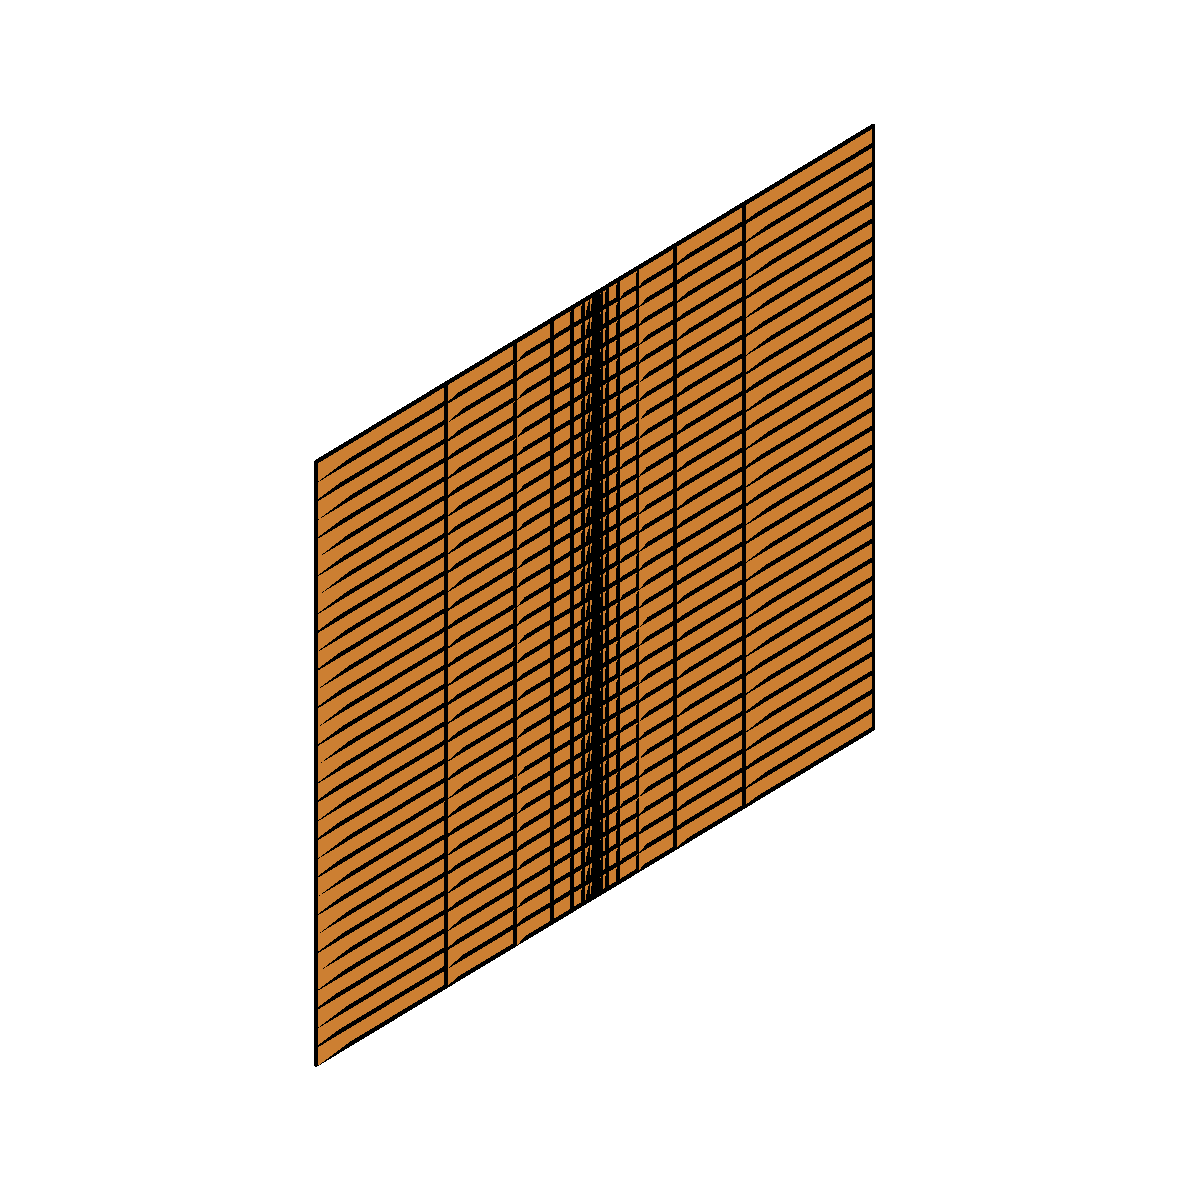
\includegraphics[width=8cm]{Images/3HelFixedu.eps}
   \caption{3-Helicoid with Fixed u}
   \label{fig:3HelFixedu}
\end{figure}

Similarly if we fix v (arbitrarily at $1$) and again ignore the third coordinate function leaving

\begin{displaymath}
\mathbf X(u,w) = (\sinh \: 1\: cos \: u, \sinh \:1 \: \sin \:\ u, w)
\end{displaymath}

This gives a cylinder whose radius increases if we increase the fixed value of v. This can be be seen in Figure \ref{fig:3HelFixedv}.
\begin{figure}[htbp]
	\centering
       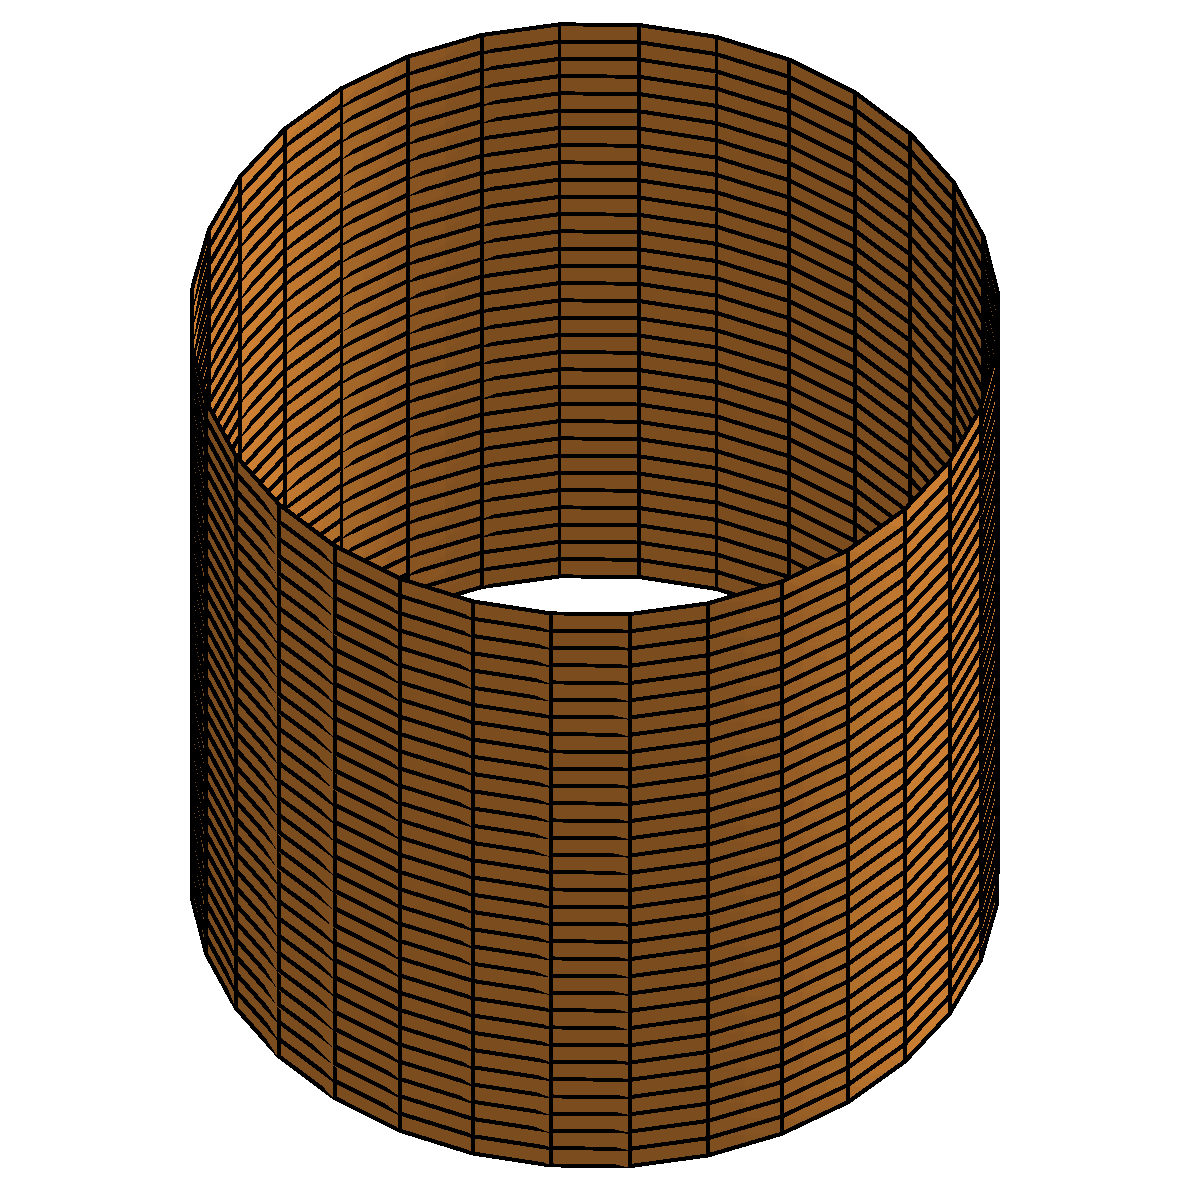
\includegraphics[width=8cm]{Images/3HelFixedv.eps}
   \caption{3-Helicoid with Fixed v}
   \label{fig:3HelFixedv}
\end{figure}


\newpage
\section{Conclusion}
The first half of this project was concerned with minimal surfaces in their classical $\mathbb R^3$ setting. We saw minimal surfaces in their real world soap film origins before introducing Differential Geometry, and noting that all Minimal Surfaces have zero mean curvature.

Having this property that characterised all minimal surfaces allowed us to set up a partial differential equation known as the Minimal Surface Equation, at which point we imposed various algebraic and geometric constraints in order to be able to solve the equation and find Minimal Surfaces. Although this approach gave some nice results; notably that the Helicoid is the only ruled minimal surface and the Catenoid is the only minimal surface of rotation, it failed to provide large numbers of different surfaces since it hinges on being able to solve the related partial differential equations which often proves too difficult.

 In order to continue our exploration of these surfaces we therefore looked to complex analysis. The power of complex analysis opened up the underlying beauty of minimal surfaces - their harmonic conjugate families, isothermal parameters that simplify the equations, deep links between minimal surfaces and the Gauss Map and of course the jewel that is the \emph{Weierstrass-Enneper Representation} which allows us to produce new minimal surfaces virtually at will.

Having laid down this classical base for minimal surfaces we then left the confines of $\mathbb R^3$ and looked at an example of how the $\mathbb R^3$ result, showing that the only minimal ruled surface is the Helicoid, generalises to hypersurfaces in higher dimensions. This required a large amount of Riemannian Manifold geometry which has proved fascinating.

Whenever possible, illustrations of the surfaces considered have been included. These were produced in Maple and whilst obviously nice to look at, it is important to realise that this relatively recent computer aided tool for rendering surfaces has been responsible for the rapid advances in the field in recent decades. Such images do not provide solid mathematical proof however they can provide the impetus to make statements which the mathematician can then attempt to prove. A prime example of this was the discovery in 2004 of an \emph{Embedded Genus One Helicoid} (a Helicoid with a handle). Computer visualisation was used to suggest the existence of such an object. However a computer has no way of knowing whether somewhere out towards infinity the surface would intersect itself. Therefore it was left to mathematicians to prove that this surface was in fact embedded. See \cite{HOFF}

Of course there is a huge wealth of material on minimal surfaces that we have not touched upon. It would have been nice to provide an overview of the calculus of variations to approach minimal surfaces and show that they do in fact form at turning points of surface area. A treatment of this can be found in \cite{OPR}. Also minimal surfaces are part of a much larger group of surfaces known as \emph{Constant Mean Curvature Surfaces}. As the name suggests these are surfaces that have mean curvature of a fixed value. The list of interesting topics in this area is virtually endless.

\newpage
\newpage
\appendix

\section{Maple Code Snippets}

Following are code snippets that help with the exploration of minimal surfaces in three space. All code is written in Maple 10 but mostly should be backward compatible. For virtually all cases you will need the following in your header:

\begin{verbatim}
restart;
with(LinearAlgebra);
with(VectorCalculus);
with(plots);
\end{verbatim}

\subsection{Harmonic Conjugate}
The following program takes a function of variables u and v. If it is a harmonic function it will return it's harmonic conjugate if it is not it will inform you that your function is not harmonic. Note that it will not accept a vector, you must deal with each coorodinate component seperatly. Eg If your surface is defined $\mathbf X(u,v) := X_1(u,v) \mathbf e_x + X_2(u,v) \mathbf e_y + X_3(u,v) \mathbf e_z$ you would run ConjHarmonic 3 times with eg \verb|ConjHarmonic(X[1]);|

\begin{verbatim}
ConjHarmonic := proc (X) 
    
local harm, VnoK, K, V; 
harm := (diff(X, u, u))+(diff(X, v, v)); 
if harm = 0 then YnoK := int(diff(X, u), v); 
	Ku := -(diff(X, v))-(diff(YnoK, u)); 
	Y := YnoK+int(Ku, u); 
	RETURN(Y);
else 
	RETURN(0);
end if; 
    
end proc;
\end{verbatim}

\newpage

\subsection{Weierstrass-Enneper Representations}
This takes two functions of the complex variable z and an output selector. Using defintions from section \ref{WERep}: 1 Returns $\mathbf X$, 2 Returns $\mathbf Y$, 3 Returns $\mathbf \Phi$. 

\begin{verbatim}
WERep := proc(f,g,select)
    
local X, Y, Z, Phi;
assume(u, 'real');
assume(v, 'real');

Z:=Vector(3); 
Z[1] := int(f*(1-g^2), z);
Z[2] := int(I*f*(1+g^2), z);
Z[3] := int(2*f*g, z);

X:=Vector(3);
X[1] := simplify(Re(expand(subs(z=u+I*v, Z[1]))),'symbolic');
X[2] := simplify(Re(expand(subs(z=u+I*v, Z[2]))),'symbolic');
X[3] := simplify(Re(expand(subs(z=u+I*v, Z[3]))),'symbolic');

Y:=Vector(3);
Y[1] := simplify(Im(expand(subs(z=u+I*v, Z[1]))),'symbolic');
Y[2] := simplify(Im(expand(subs(z=u+I*v, Z[2]))),'symbolic');
Y[3] := simplify(Im(expand(subs(z=u+I*v, Z[3]))),'symbolic');

Phi:=Vector(3);
Phi[1] := simplify(subs(z=u+I*v, f*(1-g^2)),'symbolic');
Phi[2] := simplify(subs(z=u+I*v, I*f*(1+g^2)),'symbolic');
Phi[3] := simplify(subs(z=u+I*v, 2*f*g),'symbolic');

if select = 1 then
	RETURN(X);
elif select = 2 then
	RETURN(Y);
elif select = 3 then
	RETURN(Phi);
else
	RETURN("Error - Bad Output Selector!")
end if;

end proc;
\end{verbatim}

\newpage
\begin{thebibliography}{99}

\bibitem[BCA]{BCA} Jerrold E. Marsden, Michael J. Hoffman, Basic Complex Analysis, 0-7167-1814-6

\bibitem[BLR]{BLR} D.E.Blair \& J.R.Vanstone, A Generalization of the Helicoid

\bibitem[DoC]{DoC} Manfredo P. Do Carmo, Differential Geometry of Curves and Surfaces, Prentice-Hall, Inc (1976)

\bibitem[EDG]{EDG} Andrew Pressley, Elementary Differential Geometry, Springer undergraduate mathematics series, 1-8523-3152-6

\bibitem[HIC]{HIC} N.J. Hicks, Notes on Differential Geometry 

\bibitem[MT]{MT}  J. Marsden and A. Tromba, Vector Calculus, W.H. Freeman, 1988

\bibitem[MUN]{MUN} http://www.strobel-fotoservices.de/

\bibitem[HOFF]{HOFF} Matthias Weber, David Hoffman, Michael Wolf, An embedded genus-one helicoid

\bibitem[OPR]{OPR} John Oprea, The Mathematics of Soap Films: Explorations with Maple, AMS, 0-8218-2118-0

\bibitem[OSS]{OSS} R. Osserman, A Survey of Minimal Surfaces, Dover, 1986

\bibitem[WOL]{WOL} http://mathworld.wolfram.com/

\end{thebibliography}

\begin{itemize}
\item All surfaces were rendered using Maple\textsuperscript{\textsc{tm}}.
\item All diagrams were drawn using Adobe Illustrator\textsuperscript{\textsc{tm}}.
\item This project was typeset with \LaTeX.
\end{itemize}

\end{document}

